% Arquivo LaTeX de exemplo de dissertação/tese a ser apresentados à CPG do IME-USP
%
% Versão 5: Sex Mar  9 18:05:40 BRT 2012
%
% Criação: Jesús P. Mena-Chalco
% Revisão: Fabio Kon e Paulo Feofiloff
%
% Obs: Leia previamente o texto do arquivo README.txt

\documentclass[11pt,twoside,a4paper]{book}

% ---------------------------------------------------------------------------- %
% Pacotes
\usepackage[T1]{fontenc}
\usepackage[brazil]{babel}
\usepackage[utf8]{inputenc}
\usepackage[pdftex]{graphicx}           % usamos arquivos pdf/png como figuras
\usepackage{setspace}                   % espaçamento flexível
\usepackage{indentfirst}                % indentação do primeiro parágrafo
\usepackage{makeidx}                    % índice remissivo
\usepackage{float}
\usepackage[nottoc]{tocbibind}          % acrescentamos a bibliografia/indice/conteudo no Table of Contents
\usepackage{courier}                    % usa o Adobe Courier no lugar de Computer Modern Typewriter
\usepackage{type1cm}                    % fontes realmente escaláveis
\usepackage{listings}                   % para formatar código-fonte (ex. em Java)
\usepackage{titletoc}
\usepackage{amsfonts}
\usepackage{amssymb}
\usepackage{amsmath}
%\usepackage[bf,small,compact]{titlesec} % cabeçalhos dos títulos: menores e compactos
\usepackage[fixlanguage]{babelbib}
\usepackage[font=small,format=plain,labelfont=bf,up,textfont=it,up]{caption}
\usepackage{subcaption}
\usepackage[usenames,svgnames,dvipsnames]{xcolor}
\usepackage[a4paper,top=2.54cm,bottom=2.0cm,left=2.0cm,right=2.54cm]{geometry} % margens
%\usepackage[pdftex,plainpages=false,pdfpagelabels,pagebackref,colorlinks=true,citecolor=black,linkcolor=black,urlcolor=black,filecolor=black,bookmarksopen=true]{hyperref} % links em preto
\usepackage[pdftex,plainpages=false,pdfpagelabels,pagebackref,colorlinks=true,citecolor=DarkGreen,linkcolor=NavyBlue,urlcolor=DarkRed,filecolor=green,bookmarksopen=true]{hyperref} % links coloridos
\usepackage[all]{hypcap}                    % soluciona o problema com o hyperref e capitulos
\usepackage[round,sort,nonamebreak]{natbib} % citação bibliográfica textual(plainnat-ime.bst)
\bibpunct{(}{)}{;}{a}{\hspace{-0.7ex},}{,} % estilo de citação. Veja alguns exemplos em http://merkel.zoneo.net/Latex/natbib.php

\fontsize{60}{62}\usefont{OT1}{cmr}{m}{n}{\selectfont}

% ---------------------------------------------------------------------------- %
% Cabeçalhos similares ao TAOCP de Donald E. Knuth
\usepackage{fancyhdr}
\pagestyle{fancy}
\fancyhf{}
\renewcommand{\chaptermark}[1]{\markboth{\MakeUppercase{#1}}{}}
\renewcommand{\sectionmark}[1]{\markright{\MakeUppercase{#1}}{}}
\newcommand{\source}[1]{\caption*{Source: {#1}} }
\renewcommand{\headrulewidth}{0pt}

% ---------------------------------------------------------------------------- %
\graphicspath{{./figuras/}}             % caminho das figuras (recomendável)
\frenchspacing                          % arruma o espaço: id est (i.e.) e exempli gratia (e.g.)
\urlstyle{same}                         % URL com o mesmo estilo do texto e não mono-spaced
\makeindex                              % para o índice remissivo
\raggedbottom                           % para não permitir espaços extra no texto
\fontsize{60}{62}\usefont{OT1}{cmr}{m}{n}{\selectfont}
\cleardoublepage
\normalsize

% ---------------------------------------------------------------------------- %
% Opções de listing usados para o código fonte
% Ref: http://en.wikibooks.org/wiki/LaTeX/Packages/Listings
\lstset{ %
language=C,                  % choose the language of the code
basicstyle=\footnotesize,       % the size of the fonts that are used for the code
numbers=left,                   % where to put the line-numbers
numberstyle=\footnotesize,      % the size of the fonts that are used for the line-numbers
stepnumber=1,                   % the step between two line-numbers. If it's 1 each line will be numbered
numbersep=5pt,                  % how far the line-numbers are from the code
showspaces=false,               % show spaces adding particular underscores
showstringspaces=false,         % underline spaces within strings
showtabs=false,                 % show tabs within strings adding particular underscores
frame=single,                   % adds a frame around the code
framerule=0.6pt,
tabsize=2,                      % sets default tabsize to 2 spaces
captionpos=b,                   % sets the caption-position to bottom
breaklines=true,                % sets automatic line breaking
breakatwhitespace=false,        % sets if automatic breaks should only happen at whitespace
escapeinside={\%*}{*)},         % if you want to add a comment within your code
backgroundcolor=\color[rgb]{1.0,1.0,1.0}, % choose the background color.
rulecolor=\color[rgb]{0.8,0.8,0.8},
extendedchars=true,
xleftmargin=10pt,
xrightmargin=10pt,
framexleftmargin=10pt,
framexrightmargin=10pt
}

% ---------------------------------------------------------------------------- %
% Corpo do texto
\begin{document}
\frontmatter
% cabeçalho para as páginas das seções anteriores ao capítulo 1 (frontmatter)
\fancyhead[RO]{{\footnotesize\rightmark}\hspace{2em}\thepage}
\setcounter{tocdepth}{2}
\fancyhead[LE]{\thepage\hspace{2em}\footnotesize{\leftmark}}
\fancyhead[RE,LO]{}
\fancyhead[RO]{{\footnotesize\rightmark}\hspace{2em}\thepage}

\onehalfspacing  % espaçamento

% ---------------------------------------------------------------------------- %
% CAPA
% Nota: O título para as dissertações/teses do IME-USP devem caber em um
% orifício de 10,7cm de largura x 6,0cm de altura que há na capa fornecida pela SPG.
\thispagestyle{empty}
\begin{center}
    \vspace*{2.3cm}
    \textbf{\Large{Aceleração de Registro Não-Rígido de Imagens em GPU}}\\

    \vspace*{1.2cm}
    \Large{Thiago de Gouveia Nunes}

    \vskip 2cm
    \textsc{
    Dissertação apresentada\\[-0.25cm]
    ao\\[-0.25cm]
    Instituto de Matemática e Estatística\\[-0.25cm]
    da\\[-0.25cm]
    Universidade de São Paulo\\[-0.25cm]
    para\\[-0.25cm]
    obtenção do título\\[-0.25cm]
    de\\[-0.25cm]
    Mestre em Ciências}

    \vskip 1.5cm
    Programa: Ciência da Computação\\
    Orientador: Prof. Dr. Marcel Parolin Jackowski

    \vskip 1cm
    \normalsize{Durante o desenvolvimento deste trabalho o autor recebeu auxílio
    financeiro da CAPES}

    \vskip 0.5cm
    \normalsize{São Paulo, fevereiro de 2015}
\end{center}

% ---------------------------------------------------------------------------- %
% Página de rosto (SÓ PARA A VERSÃO DEPOSITADA - ANTES DA DEFESA)
% Resolução CoPGr 5890 (20/12/2010)
%
% IMPORTANTE:
%   Coloque um '%' em todas as linhas
%   desta página antes de compilar a versão
%   final, corrigida, do trabalho
%
%
\newpage
\thispagestyle{empty}
    \begin{center}
        \vspace*{2.3 cm}
        \textbf{\Large{Aceleração de Registro Não-Rígido de Imagens em GPU}}\\
        \vspace*{2 cm}
    \end{center}

    \vskip 2cm

    \begin{flushright}
  Esta é a versão original da dissertação/tese elaborada pelo\\
  candidato Thiago de Gouveia Nunes, tal como \\
  submetida à Comissão Julgadora.
    \end{flushright}

\pagebreak


% ---------------------------------------------------------------------------- %
% Página de rosto (SÓ PARA A VERSÃO CORRIGIDA - APÓS DEFESA)
% Resolução CoPGr 5890 (20/12/2010)
%
% Nota: O título para as dissertações/teses do IME-USP devem caber em um
% orifício de 10,7cm de largura x 6,0cm de altura que há na capa fornecida pela SPG.
%
% IMPORTANTE:
%   Coloque um '%' em todas as linhas desta
%   página antes de compilar a versão do trabalho que será entregue
%   à Comissão Julgadora antes da defesa
%
%
% \newpage
% \thispagestyle{empty}
%     \begin{center}
%         \vspace*{2.3 cm}
%         \textbf{\Large{Título do trabalho a ser apresentado à \\
%         CPG para a dissertação/tese}}\\
%         \vspace*{2 cm}
%     \end{center}

%     \vskip 2cm

%     \begin{flushright}
%   Esta versão da dissertação/tese contém as correções e alterações sugeridas\\
%   pela Comissão Julgadora durante a defesa da versão original do trabalho,\\
%   realizada em 14/12/2010. Uma cópia da versão original está disponível no\\
%   Instituto de Matemática e Estatística da Universidade de São Paulo.

%     \vskip 2cm

%     \end{flushright}
%     \vskip 4.2cm

%     \begin{quote}
%     \noindent Comissão Julgadora:

%     \begin{itemize}
%       \item Profª. Drª. Nome Completo (orientadora) - IME-USP [sem ponto final]
%       \item Prof. Dr. Nome Completo - IME-USP [sem ponto final]
%       \item Prof. Dr. Nome Completo - IMPA [sem ponto final]
%     \end{itemize}

%     \end{quote}
% \pagebreak


\pagenumbering{roman}     % começamos a numerar

% Resumo
\chapter*{Resumo}

\noindent Nunes, T. G. - \textbf{Aceleração de Registro Não-Rígido de Imagens em GPU}.
2015.
Qualificação (Mestrado) - Instituto de Matemática e Estatística,
Universidade de São Paulo, São Paulo, 2015.
\\

O alinhamento geométrico, comumente conhecido como registro de imagens, é uma etapa essencial em várias
aplicações na área de processamento de imagens, que incluem desde análises populacionais na área
médica até reconstrução de mapas utilizando imagens de satélite. Deformações não rígidas representam
uma ampla gama das possíveis deformações presentes nas várias categorias de imagens que são registradas.
Atualmente, estudos que envolvem milhares de imagens estão se tornando cada vez mais comuns, sugerindo
que técnicas de aceleração sejam desenvolvidas de forma a minimizar o
tempo de análise e processamento. Como as técnicas de registro não-rígido são tradicionalmente custosas
computacionalmente, o uso de \textit{graphic processing units} (GPUs) possibilita a
aceleração das diversas etapas do processo via hardware, tais como a extração de características,
determinação de correspondências e cálculo das funções de deformação. Este trabalho
tem como objetivo a paralelização de técnicas de registro não-rígido aplicadas à arquiteturas modernas de
GPU, e avaliação de sua eficiência.
\\

\noindent \textbf{Palavras-chave:} Registro de Imagens, Thin Plate Splines, Demons, \textit{Graphic Processing Units}.

% ---------------------------------------------------------------------------- %
% Abstract
\chapter*{Abstract}
\noindent Nunes, T. G. - \textbf{Acceleration of Non-Rigid Image Registration in GPU}.
2015.
Qualificação (Mestrado) - Instituto de Matemática e Estatística,
Universidade de São Paulo, São Paulo, 2015.
\\
Geometrical image alignment, commonly known as image registration, is an essential step in a number of image processing applications,
ranging from populational studies in medical imaging to map reconstruction based on satellite images. Non-rigid deformations
represent a big slice of all possible deformations in images that need to be registered.
Presently, studies that involve thousands of images are becoming commonplace,
suggesting that acceleration techniques should be developed to diminish the analysis or processing time.
Registration techniques are usually very computational demanding, hence the use of \textit{graphic processing units} (GPUs)
creates a possibility to speedup several stages of the registration process, such as extraction of features,
determination of feature correlation and calculaton of the deformation function. This project targets the
parallelization of non-rigid registration techniques in modern GPU architecture and evaluate their
efficiency.
\\

\noindent \textbf{Keywords:} Image Registration, Thin Plate Splines, Demons, Graphic Processing Units.

% ---------------------------------------------------------------------------- %
% Sumário
\tableofcontents    % imprime o sumário

% ---------------------------------------------------------------------------- %
\chapter{Lista de Abreviaturas}
\begin{tabular}{ll}
        TPS         & \textit{Thin Plate Splines}\\
        GPU         & Unidades de Processamento Gráfico (\textit{Graphic Processing Units})\\
        GPGPU       & Computação Genérica em GPUs (\textit{General-purpose computing on graphics processing units})\\
        CUDA        & \textit{Compute Unified Device Architecture}\\
        IA          & Imagem Alvo \\
        IR          & Imagem Referência \\
\end{tabular}

% ---------------------------------------------------------------------------- %
\chapter{Lista de Símbolos}
\begin{tabular}{ll}
        $n_l$   & Número de Linhas de uma imagem \\
        $n_c$   & Número de Colunas de uma imagem \\
        $n_p$   & Número de Cortes de uma imagem \\
        $N$     & Tamanho da imagem \\
        $x$     & Variável usada para acessar a $n$-ésima linha de uma imagem \\
        $y$     & Variável usada para acessar a $n$-ésima coluna de uma imagem \\
        $n_{cp}$  & Número de características em uma imagem \\
\end{tabular}

% ---------------------------------------------------------------------------- %
% Listas de figuras e tabelas criadas automaticamente
\listoffigures
\listoftables

% ---------------------------------------------------------------------------- %
% Capítulos do trabalho
\mainmatter

% cabeçalho para as páginas de todos os capítulos
\fancyhead[RE,LO]{\thesection}

\singlespacing              % espaçamento simples
%\onehalfspacing            % espaçamento um e meio

%% ------------------------------------------------------------------------- %%
\chapter{Introdução}
\label{cap:introducao}

	



Falar sobre
gigapixel - o que é em linhas gerais, onde começou, onde é usado
registro - áreas que usam registro, como ele é usado
registtro + gigapixel - o problema de desempenho, como resolver.

% \emph{Thesis are random access. Do NOT feel obliged to read a thesis from beginning to end.}

%% ------------------------------------------------------------------------- %%
\section{Trabalhos Relacionados}
\label{sec:objetivo}

%% ------------------------------------------------------------------------- %%
\section{Organização do Trabalho}
\label{sec:organizacao_trabalho}

No Capítulo~\ref{cap:conceitos}, apresentamos o que é Registro, Unidade de Processamento Gráfico, GPGPU e os algoritmos 
de registro escolhidos. No Capítulo \ref{cap:resultados} os testes utilizados e os resultados dos dois algoritmos 
escolhidos são apresentados. Finalmente, no Capítulo~\ref{cap:conclusoes} analisamos os resultados obtidos         % associado ao arquivo: 'cap-introducao.tex'
%% ------------------------------------------------------------------------- %%
\chapter{Conceitos}
\label{cap:conceitos}

%% ------------------------------------------------------------------------- %%
\section{Registro}\index{Registro}
\label{sec:fundamentos}

    O registro de imagens tem como objetivo encontrar um alinhamento entre duas imagens diferentes. Dada duas imagens, 
a imagem Referência (R) e a imagem Alvo (A), os algoritmos de registro encontram um campo
vetorial de deslocamento que é aplicado a imagem Alvo, movendo seus pixels para um estado no qual ela esteja alinhada
com a imagem Referência. Para encontrar um alinhamento, supomos que a imagem Alvo sofreu algum tipo de deformação,
e queremos, dado algum modelo que aproxime a deformação, encontrar os parâmetros para uma função de
transformação que nos leve da imagem Alvo para a imagem Registrada, que nada mais é que a imagem Alvo alinhada a imagem
Referência.

Podemos definir o processo de registro com a seguinte equação, como \cite{brown1992survey} fez em seu estudo:
\begin{align}\label{eq:defregistro}
    R(x,y) = g(A(f(x,y)))
\end{align}
    Representamos uma imagem como uma matriz de pixels e acessamos seus pixels utilizando a seguinte convenção $R(x,y)$ 
que nos dá o pixel da imagem $R$ na posição $(x,y)$. $f(x,y) = (x',y')$ é uma função que representa o deslocamento do 
campo vetorial encontrado pelo registro e $g$ é uma função que modifica a intensidade dos pixels, se for necessário.
Cada algoritmo de registro utiliza um método diferente para encontrar a função de transformação $f$, mas os passos gerais são:
\begin{enumerate}
    \item Pré-processamento;
    \item Detecção de características;
    \item Correspondência de características;
    \item Estimativa da função de transformação;
    \item Reamostragem da imagem Alvo.
\end{enumerate} % TODO: Colocar o diagrama aqui %
    É importante salientar que nem todos algoritmos de registro seguem essa lista a risca, e mesmo que sigam eles ainda
podem realizar mais de um passo por vez. Os passos gerais são representados na imagem \ref{fig:regExplicacao}. 
Vamos tratar brevemente dos passos nas seções a seguir, explicitando em alguns pontos onde os passos podem ser acelerados,
principalmente pela paralelização de suas operações.

\begin{figure}[h]
    \centering
    \begin{subfigure}[t]{0.3\textwidth}
      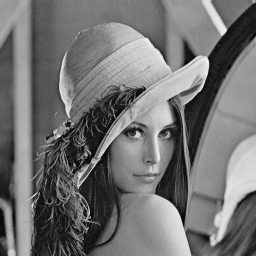
\includegraphics[width=\textwidth]{figuras/static.png}
      \subcaption*{(a)}
      \label{fig:ref-image}
    \end{subfigure}
    \begin{subfigure}[t]{0.3\textwidth}
      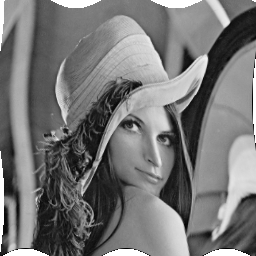
\includegraphics[width=\textwidth]{figuras/leiaMoving.png}
      \subcaption*{(b)}
      \label{fig:sin-image}
    \end{subfigure} \\
    \begin{subfigure}[t]{0.64\textwidth}
      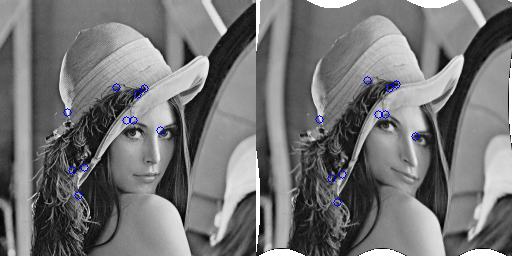
\includegraphics[width=\textwidth]{figuras/Features.png}
      \subcaption*{(c)}
      \label{fig:dist-image}
    \end{subfigure} \\
    \begin{subfigure}[t]{0.64\textwidth}
      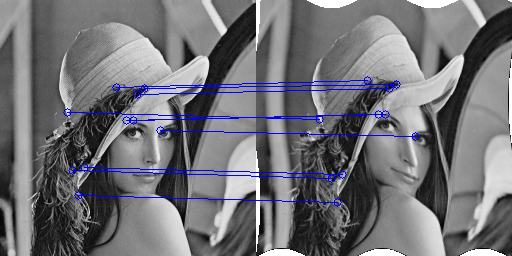
\includegraphics[width=\textwidth]{figuras/MatchedFeatures.png}
      \subcaption*{(d)}
      \label{fig:dist-image}
    \end{subfigure} \\
    \begin{subfigure}[t]{0.3\textwidth}
      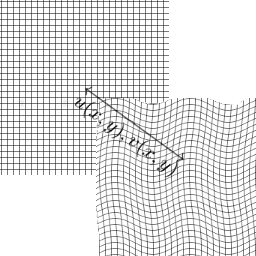
\includegraphics[width=\textwidth]{figuras/estimativa.png}
      \subcaption*{(e)}
      \label{fig:dist-image}
    \end{subfigure} 
    \begin{subfigure}[t]{0.3\textwidth}
      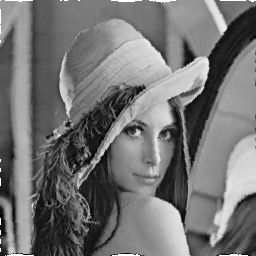
\includegraphics[width=\textwidth]{figuras/leiaRegistrada.png}
      \subcaption*{(f)}
      \label{fig:dist-image}
    \end{subfigure}
    \caption{(a) imagem Referência. (b) imagem Alvo deformada pela função seno. 
             (c) Detecção de características. (d) Correspondência de características.
             (e) Estimativa da função de transformação. (f) Reamostragem da imagem Alvo.}
    \label{fig:regExplicacao}
\end{figure}

%% ------------------------------------------------------------------------- %%
\subsection{Pré-processamento}
    Essa é a etapa mais aberta dentre todas, já que sua aplicação é totalmente dependente do problema a ser resolvido. 
Antes de iniciar o processo de registro, é possível que as imagens tenham que passar por algum processamento para 
melhorar o resultado final do registro. O pré-processamento muda de acordo com as necessidades de cada caso. Caso as
imagens tenham muito ruído, essa é a hora de aplicar filtros para melhorar sua qualidade, como um filtro Passa Alta ou 
o Passa Baixa. Certos algoritmos de registro não trabalham com as imagens, e sim com segmentações delas ou somente com 
suas bordas, então é necessário aplicar algoritmos como o \textit{Watershed}, introduzido por 
\cite{vincent1991watersheds} ou o \textit{Canny}, desenvolvido por \cite{canny1986computational}, para obter as 
segmentações e bordas, respectivamente.

%% ------------------------------------------------------------------------- %%
\subsection{Detecção de características}\index{Detecção de características}
\label{sec:dec_corr_carac}

    Com as imagens já pré-processadas, o primeiro passo para um algoritmo de registro é a localização de estruturas de 
destaque na cena ou objeto dentro das imagens. Essas estruturas são nomeadas de características, e são construidas a 
partir de um conjunto de pixels. Características devem ser facilmente identificadas, independente de variações na 
aquisição das fotografias, como mudanças na angulação ou perspectiva. Elas são separadas em 3 grupos, baseando-se nas 
suas propriedades:

\textbf{Características de Região} - As características de Região são áreas de uma imagem que apresentam uma diferença
significativa de contraste em relação a áreas vizinhas. Lagos, florestas ou regiões urbanas são exemplos desse tipo de 
característica. Elas são identificadas utilizando algoritmos de segmentação, e normalmente são representadas por um
conjunto conexo de pixels ou utilizando um \textit{template} de formato retângular ou circular centrado no centro de 
massa da Região.

\textbf{Características de Retas} - Essas características são definidas como a interface entre duas regiões de uma 
imagem, comumente chamadas de bordas. Exemplos comuns de características de Reta são ruas, rios ou o litoral, onde 
podemos claramente visualizar a diferença de intensidade, por exemplo, do mar e da areia. Métodos clássicos de detecção 
de bordas como o Canny ou o filtro laplaciano são usados para identificar essas características.

\textbf{Características de Ponto} - São pontos de intersecção entre linhas, representados por intersecções de ruas ou
rios, ou pontos de máxima curvatura. Algoritmos para identificação de pontos utilizam técnicas mais avançadas, dada a 
dificuldade de encontrá-los. Os mais básicos encontram as intersecções de linhas enquanto os mais avançados buscam
centroides de regiões ou o máximo local de uma \textit{wavelet}.

  Encontrar características em imagens é um passo não só de registro de imagens, mas em aprendizagem computacional, por
exemplo reconhecimento de padrões. Dada essa importância, vários algoritmos foram desenvolvidos com o passar dos anos 
para resolver de maneira rápida e eficiente a detecção de características. Falaremos sobre dois métodos firmados 
no meio científico, o \textit{Scale Invariant Feature Transform} (SIFT) , introduzido por \cite{lowe1999object}, e o 
\textit{Speeded Up Robust Features} (SURF), desenvolvido por \cite{bay2006surf}. Como esse métodos fazem tanto a captura
das característica quanto a correspondência entre elas falamos sobre eles na próxima seção.

%% ------------------------------------------------------------------------- %%
\subsection{Correspondência de características}\index{Correspondência de características}

    Com as características de cada uma das imagens encontradas, o próximo passo é realizar a correspondência entre elas.
A função desse passo é encontrar a correspondência entre pontos da imagem Referência para a imagem Alvo, ou vice-versa. 
O processo pode ser realizado tanto escolhendo ponto a ponto da imagem Referência e procurando o ponto com maior valor 
de proximidade entre os pontos da imagem Alvo, quanto utilizando métodos estatísticos para determinar quais pontos são 
correspondentes entre as duas imagens. É importante que esse passo consiga identificar pontos físicos, com coordenadas, 
em cada par de características, para que uma primeira estimativa dos parâmetros da função de transformação possa ser 
utilizada como ponto de partida para o próximo passo.

    A primeira solução a ser apresentada, a \textbf{Correspondência por Área}, mescla o passo de Detecção com o de 
Correspondência. Esse método utiliza duas janelas, uma em cada imagem, com formato retangular ou circular, aplicando
métricas em cada uma das janelas com a finalidade de calcular a relação entre as janelas. O algoritmo segue realizando
esse cálculo para todas as combinações possíveis de janelas entre as duas imagens, e sempre que um máximo é encontrado
o centro das janelas são usados para marcar a correspondência. Várias métricas podem ser utilizadas, como a 
Correlação entre as intensidades das janelas, o estudo do espectro da transformada de \textit{Fourier} das janelas ou 
o cálculo da informação mútua entre elas.

    A descoberta de correspondência entre \textbf{Características de Região} é feita utilizando, principalmente, duas 
técnicas. A primeira, mais simples na sua ideia, é parear regiões da imagem Referência com a região da imagem Alvo a 
qual tenha o contorno mais parecido possível. Os métodos que fazem esse pareamento devem ser capazes de encontrar os 
pares mesmo que eles tenham sofrido rotações ou mudança de escala. Descritores de Fourier e representações matriciais 
das regiões são exemplos de métodos usados para realizar a correspondência entre características de região.

    Os métodos para encontrar correspondências entre \textbf{Características de Retas} tem as mesmas restrições que os
de Região, ou seja, devem conseguir realizar o pareamento de linhas que sofreram rotação, mudança de escala ou 
translação. O primeiro passo de um algoritmo é comparar as retas da imagem Referência com todas as possíveis rotações 
de todas as retas da imagem Alvo. Quando um possível par é encontrado, um valor de correspondência é calculado, 
utilizando um peso maior para a direção da reta, algo que não sofre tanta influência de ruído, e um peso menor para 
atributos como comprimento e largura, que são influenciados pelo ruído. O algoritmo ainda deve ser capaz de parear mais 
de duas retas por vez, dada a possibilidade de uma reta em uma das imagens ser representada por duas retas na outra 
imagem.

    Por fim, as correspondências entre \textbf{Características de Ponto} podem ser encontradas utilizando-se várias 
técnicas distintas. Como o número e o agrupamento de pontos geralmente não muda tanto com rotações e translações de 
imagens, métodos de \textit{Clustering} são usados para parear pontos. Os \textit{Clusters} são montados com base na 
proximidade dos parâmetros de uma transformação que leve pontos da imagem Alvo para pontos da imagem Referência. Outro 
método define as características através de descritores invariantes que podem obedecer a 4 regras: \textbf{Invariância}, 
características correspondentes devem ter os mesmos descritores; \textbf{Unicidade}, características diferentes devem 
ter descritores diferentes; \textbf{Estabilidade}, os descritores devem deformar de maneira proporcional a deformação
aplicada na imagem; e \textbf{Independência}, se o descritor for representado por um vetor, seus componentes devem ser 
independentes. O que define um descritor deve ser decidido caso a caso. O modelo mais simples usado é a propria 
intensidade do pixel, e a intensidade de seus vizinhos. Outros descritores válidos são ângulos entre correspondências 
vizinhas ou a distribuição espacial dos vizinhos.

    Podemos separar os algoritmos de correspondências em dois tipos com base no estilo com que eles fazem a busca de 
correspondências. O primeiro tipo escolhe uma correspondência na imagem Referência e realiza uma busca em largura por
todas as correspondências da imagem Alvo, buscando aquela com maior relação com a da imagem Referência. Esse processo
pode ser facilmente acelerado utilizando uma paralelização com todas as correspondências da imagem Referência. Já o 
outro tipo realiza uma busca entre as relações das características e encontra os pares de maneira iterativa. A 
aceleração desse passo depende totalmente da sua implementação.

    O modelo \textit{MapReduce} apresenta uma outra alternativa para acelerar esse passo e o anterior. Ele foi 
desenvolvido por \cite{dean2008mapreduce} e pela Google. O modelo \textit{MapReduce} foi desenvolvido para realizar 
processamento em lote de um número gigantesco de dados, o popular \textit{Big Data}, dado que não exista muita diferença 
em como os dados devem ser processados. Seu modelo de programação contém duas etapas principais, o \textit{Map}, que 
recebe um par de dados e retorna um par de valor/chave. Um passo intermediário agrupa todos os valores com mesma chave e
a lista resultante é enviada para o próximo passo, o \textit{Reduce}, onde a lista é processada. O nosso \textit{Map} 
recebe uma imagem Alvo e Referência, e encontra as características delas, enquanto o processo de agrupamento encontra as
suas correspondências. O \textit{Reduce} fica com qualquer etapa de pós-processamento, se necessário.

  Abaixo falamos sobre o \textit{Scale Invariant Feature Transform} e o \textit{Speeded Up Robust Features}, que são
métodos que fazem tanto a captura quanto a correspondência de características.

\subsubsection{Scale Invariant Feature Transform (SIFT)}
  O SIFT cria, para cada característica, um vetor de propriedades inváriaveis com rotações, mudanças de escala e 
rotações, e parcialmente inváriaveis com mudanças de projeção e iluminação. O primeiro passo do algoritmo é encontrar
posições, que ele chama de \textbf{chave}, que obedeçam as propriedades acima. Para isso ele faz uma busca no espaço
de escala de uma imagem, procurando pelo máximo ou minimo da diferença de Gaussianas nesse espaço.

  O espaço de escala de uma imagem é criado construindo uma piramide de reamostragens de uma imagem. Na base temos a 
imagem original e em cada andar da piramide se encontra uma versão reamostrada da imagem. Antes de reamostrar a próxima 
imagem da piramide, o SIFT aplica 2 vezes um filtro Gaussiano com desvio padrão $\sigma = \sqrt{2}$ a imagem atual, 
criando mais duas imagens, que chamaremos de $A$ e $B$, respectivamente. A reamostragem para criar o próximo patamar da 
piramide é criado aplicando uma interpolação bilinear com espaçamento de $1.5$ pixels a imagem $B$ do patamar atual.
 
  A busca pelos minimos ou máximos da diferença de Gaussianas é feita de uma maneira não direta, com fim de otimizar
o cálculo. Primeiro, cada pixel da imagem é comparado com seus 8 vizinhos. Se ele é um minimo ou máximo então cálculamos
sua projeção na imagem abaixo, lembrando da reamostragem de $1.5$ pixels. Se ele continua sendo menor ou maior que sua 
projeção e os 8 vizinhos da projeção, o processo é repetido para a imagem acima. Os pixels que passarem por essas 
etapas são os pixels \textbf{chave}.

  Com os pontos \textbf{chave} encontrados, o algoritmo agora encontra uma orientação e magnitude para eles. Elas são
obtidas cálculando o gradiente da imagem $A$ em cada nível da piramide e obtendo a orientação e magnitude deles. Para
tornar a magnitude parcialmente inváriavel em relação a mudanças de iluminação ela é limiarizada em $0.1$ vezes o valor
da maior magnitude em um nível. A orientação é determinada utilizando um histograma criado a partir de uma Gaussiana
com desvio padrão três vezes maior que o usado no filtro da imagem $A$. Após um processo de suavização no histograma,
seu máximo é escolhido como orientação para o pixel \textbf{chave}. Para tornar o método mais robusto, o processo é
repitido para várias rotações do sistema de orientação original, para representar possíveis rotações ou deformações não
rigidas das imagens.

  Todas essas propriedades obtidas dos pontos \textbf{chave} são utilizadas para construir vetores, que serão utilizados
para realizar comparações entre características de imagens diferentes afim de encontrar as correspondências. A busca de
correspondência é feita usando uma k-d-árvore, populando ela com as características de uma das imagens.

%% ------------------------------------------------------------------------- %%
\subsection{Estimativa da função de transformação}\index{Estimativa da função de transformação}
    
Com o conjunto de correspondências encontrado pelo passo anterior, os algoritmos de registro tem uma base para 
começar o processo de estimativa da função de transformação. Cada algoritmo assume um modelo de transformação diferente
para a deformação que a imagem sofreu, como por exemplo, uma modelagem elástica, por propagação de fluidos ou uma
simples translação. Juntando a modelagem com as correspondências, os algoritmos conseguem estimar parâmetros iniciais
para a função de transformação. Utilizando alguma métrica para passear pelo espaço de parâmetros, os algoritmos encontram
algum conjunto de parâmetros que alinhe a imagem Alvo com a imagem Referência. Na seção \ref{sec:algReg}, apresentaremos
dois algoritmos estudados com enfase nessa etapa.

%% ------------------------------------------------------------------------- %%
\subsection{Reamostragem da imagem Alvo}\index{Reamostragem da imagem Alvo}

O último passo do registro é a montagem da imagem Registrada, ou a reamostragem da imagem Alvo. O passo anterior
dá um conjunto de parâmetros para a montagem da imagem final, logo esse passo tem como objetivo a aplicação
da transformação $f$ utilizando os parâmetros encontrados sob todas as posições da imagem Alvo. Temos:

\begin{align}\label{eq:reamostragem}
    F(x_i,y_j) = A(f_o(x_i,y_j))), \forall (i = 1, \dots, n_c), (j = 1, \dots, n_l)
\end{align}

    Onde $F(x_i,y_j)$ representa a posição $(x_i,y_j)$ da imagem Registrada e $f_o$ é a função $f$ sob os parâmetros
encontrados no passo anterior.

%% ------------------------------------------------------------------------- %%
%% ------------------------------------------------------------------------- %%
\section{Computação de Alto Desempenho}\index{HPC,GPGPU}\label{GPGPU}
    
    Computação de Alto Desempenho (\textit{High Performance Computing} - HPC) designa sistemas de alta capacidade de processamento
e armazenamento de dados montados especificamente resolver grandes problemas científicos, para os quais computadores pessoais não
são o suficiente. Esses sistemas variam em tamanho, poder computacional e capacidade de armazenamento. Os mais famosos,
conhecido como Supercomputadores, são máquinas montadas especialmente para resolver um único problema, ou um grupo
especifico de problemas, e tem em sua composição milhares de processadores. Porém existem instâncias mais simples de 
\textit{HPC}, onde um sistema é montado a partir de um \textit{Cluster} de computadores pessoais.

    No inicio dos anos 2000, com o inicio do suporte de operações de ponto flutuante, ainda que emuladas por software, 
e com o surgimento de um \textit{shaders} programável, as Unidades de Processamento Gráfico 
(\textit{Graphic Processing Units} - GPU) começaram a ser usadas para executar código de natureza mais genérica.
Chamamos a aplicação de GPUs na solução de problemas computacionais, fora da área de computação gráfica, 
de \textit{General-purpose computing on graphics processing units}, ou GPGPU. Com o alto custo beneficio que as GPUs 
trazem e seu alto poder de realizar processamento paralelo, arquiteturas de HPC começaram a aparecer utilizando não a 
CPU, mas sim a GPU como principal carro chefe de processamento.

\subsection{Unidade de Processamento Gráfico}
    A GPU nasceu da necessidade de renderizar cenas complexas, mantendo uma taxa de quadros por segundos
aceitável para o usuário, em tempo real. Ela foi projetada para executar uma sequência fixa de passos que transformam
os dados da cena em objetos virtuais na tela. A sequência de passos se assemelha a uma linha de montagem de fabricas,
onde objetos são montados parte por parte de forma sequencial. Chamamos essa sequência de \textit{Pipeline} gráfico 
(ver figura \ref{fig:pipeline}), e a GPU é construída para que cada passo dele seja mapeado para uma ou mais partes do 
seu hardware.

    É comum cenas conterem objetos complexos, compostos de milhões de triângulos, que passarão, um por um, pelo
\textit{Pipeline} gráfico. Para acelerar o processo de renderização, as GPUs seguem a arquitetura de Instrução Única,
Múltiplos Dados (\textit{Single Instruction, Multiple Data} - SIMD). Como o nome já diz, essa arquitetura permite que 
a mesma instrução seja executada várias vezes em paralelo utilizando instâncias de dados diferentes. A figura 
\ref{fig:simd} mostra a implementação do \textit{Pipeline} utilizando a arquitetura SIMD no hardware da GPU.
    
    Para implementar de maneira esse paradigma, a GPU é composta de vários hardwares específicos. Nela existe um 
escalonador para \textit{threads} implementado em hardware. Ele é responsável por escalonar as \textit{threads} que serão
executadas nos \textit{Streaming Multiprocessors} (SM). Um SM é um conjunto de vários processadores, um pequeno bloco de
memória própria, um cache de instruções e 8 unidades de funções gráficas.

    O código que será executado em cada processador é chamado de \textbf{kernel}. Ao executar um kernel na GPU, o 
hardware criará \textit{threads}, cada uma delas executando o mesmo código, mas com dados diferentes. Nas placas NVIDIA as \textit{threads} 
são agrupadas em blocos, e esses blocos são escalonados para cada SM. Depois, todas as \textit{threads} dentro de um bloco são 
divididas em pequenos grupos chamados de \textbf{warp}, e cada warp é executado paralelamente dentro do 
mesmo SM para qual o bloco foi escalonado. Existe um limite para a quantidade de \textit{threads} escalonadas para execução
dentro de um SM, que é definida pelos recursos que cada \textit{thread} consome. Por exemplo, não há como executar 10 \textit{threads}
que consomem 10 registradores cada em um SM com 90 registradores.

    A memória da GPU é limitada em relação à da CPU. GPUs tem, em média, 4GB
de memória, enquanto CPUs tem acesso a, no minimo, 8GB. O acesso a um mesmo bloco de memória é concorrente, mas ao utilizar caches e leitura 
ou escritas em conjunto podemos minimizar a taxa com que leituras ou escritas conflitantes são feitas. Mas ainda sim é 
necessário atenção ao escrever um kernel. Dada a estrutura do hardware da GPU, é melhor deixar \textit{threads} que façam 
operações sobre posições de memória próximas no mesmo SM, assim elas podem utilizar a memória compartilhada do mesmo, e 
elas podem requisitar em conjunto um mesmo bloco da memória principal, se necessário.

    Outro fator limitante é a transferência de dados da memória principal do computador para a memória 
principal da GPU. A transmissão é feita por um barramento PCI Express, com velocidades de até 16GB/s ( dado que o
barramento seja utilizado somente pela GPU ). Essa transmissão é a parte mais lenta de todo o
processo de execução na GPU e dado isso, em alguns casos é mais viável executar na GPU um pedaço do seu programa que 
seria executado na CPU do que retornar os dados computados na GPU para a CPU, executar esse pedaço especifico, e 
passá-los de volta para a GPU para mais operações e novamente retornar esses dados para a CPU no final, passando duas 
vezes a mais pelo PCI Express.

\begin{figure}[H]
    \centering
    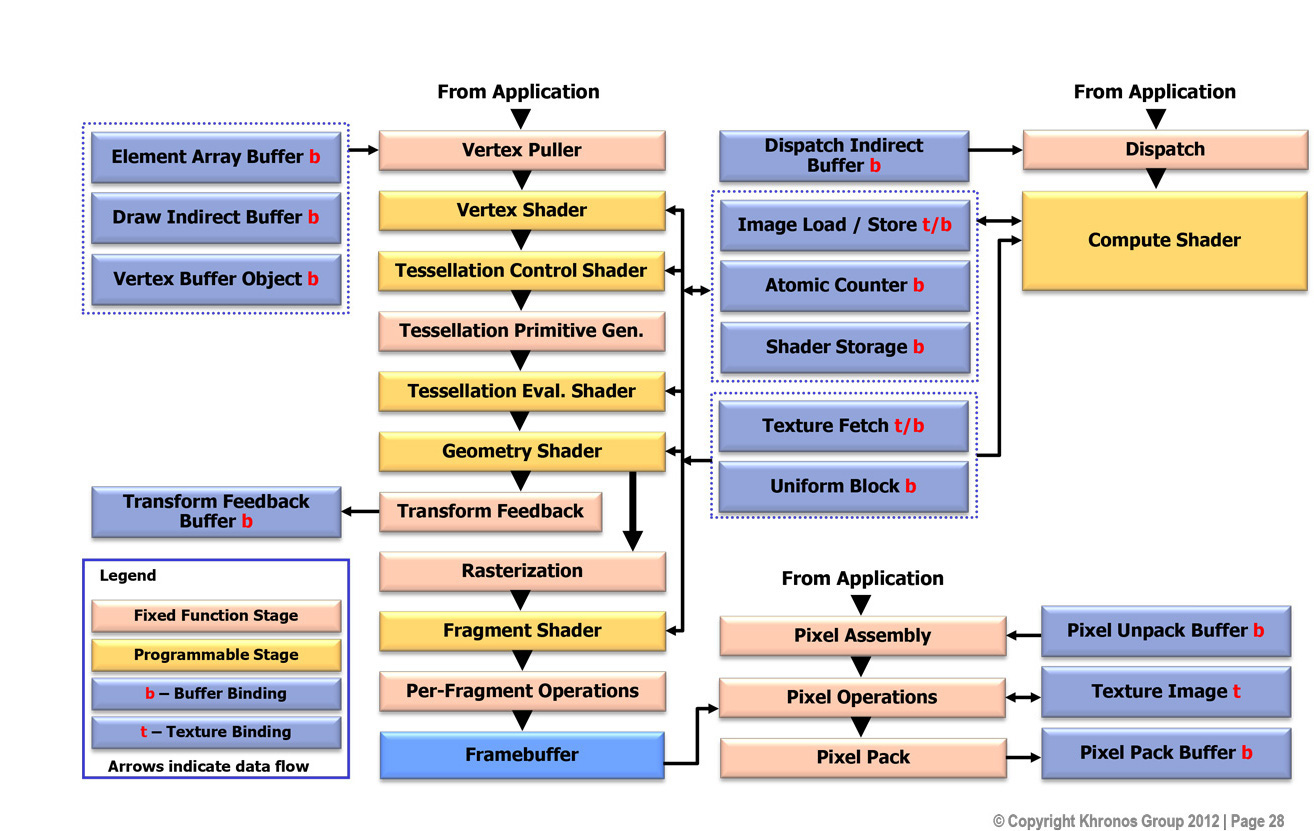
\includegraphics[width=1\textwidth]{figuras/pipeline.jpg}
    \caption{\textit{Pipeline} do OpenGL 4.x, por \citep{pipeline}. Todos os passos marcados pela cor amarela podem
    ser reprogramados para serem utilziados por aplicações GPGPU. (Modificada)}
    \label{fig:pipeline}
\end{figure}

\begin{figure}[H]
    \centering
    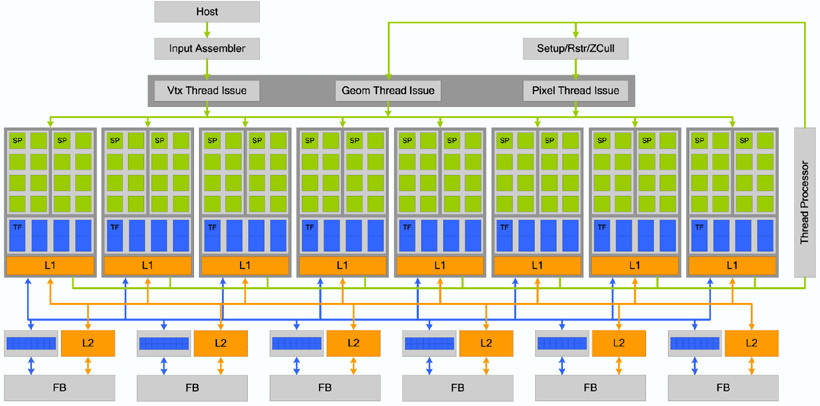
\includegraphics[width=1\textwidth]{figuras/simd.jpg}
    \caption{Arquitetura da GPU SIMD, por \citep{blythe2008rise}.}
    \label{fig:simd}
\end{figure}

\subsection{CUDA}\index{CUDA}
\textit{Compute Unified Device Architecture}, definida pela (CUDA) é uma arquitetura de programação para GPUs criada 
pela ~\cite{nvidia2007compute}.
Ele adiciona suas diretrizes para as linguagens C, C++, FORTRAN e Java, permitindo que elas usem a GPU.
Esse trabalho usa o CUDA junto com a linguagem C.
A versão 1.0 do CUDA foi disponibilizada no inicio de 2007. Atualmente só existe um compilador para CUDA, o nvcc,
e ele só da suporte para GPUs NVIDIA.

Para uma função executar na GPU ela precisa ser invocada de um programa da CPU. Chamamos esse programa de \textit{Host}
e a GPU onde o kernel irá executar de \textit{Device}.

O CUDA implementa um conjunto virtual de instruções e memória, tornando os programas retroativos. O compilador
primeiro compila o código em C para um intermediário, chamado de PTX, que depois será convertido em linguagem
de máquina. Na conversão do PTX para linguagem de máquina o compilador verifica quais instruções o \textit{device}
suporta e converte o código para usar as instruções corretas.
Para obter o maior desempenho possível, é importante saber para qual versão o código final será compilado, 
pois na passagem do código de uma versão maior para uma menor não existe a garantia que o algoritmo seguira as mesmas instruções, 
o compilador pode mudar um conjunto de instruções para outro menos eficiente, ou em alguns casos, algumas instruções não existem em
versões mais antigas do hardware.

\subsubsection{Modelo de Plataforma}
A inicialização dos recursos que o CUDA necessita para a comunicação com a GPU é feita no background da
aplicação no momento da primeira chamada de alguma das diretivas do CUDA. Essa primeira diretiva terá um
tempo maior de execução que chamadas subsequentes a mesma diretiva. Na inicialização o CUDA identifica
os \textit{devices} existentes e escolhe um deles para ser o responsável pelas execuções posteriores.

O próximo passo é a alocação de memória no \textit{device}. As operações de leitura de memória de um kernel são feitas somente
na memória de um \textit{device}. A alocação dessa memória é feita pelo \textit{host}, usando \verb#cudaMalloc()#. 
Para copiar a memória do \textit{host} para o \textit{device} ou vice-versa,
\verb#cudaMemcpy()# é usada. Para liberar o espaço alocado após a execução basta usar o \verb#cudaFree()#.
Todas essas diretivas recebem um ponteiro do \textit{host}, usado para o controle sobre qual posição da memória está sendo
operado em cada operação.

O CUDA dá suporte a alocação de vetores em duas ou três dimensões através de: \verb#cudaMallocPitch()# e 
\verb#cudaMalloc3D()#, respectivamente. É necessário usar as modificações dos comandos \verb#Memcpy# para
duas ou três dimensões também, que são: \verb#cudaMemcpy2D()#, \verb#cudaMemcpy3D()#.

\subsubsection{Modelo de Programação}
Um kernel no CUDA é uma função C que será executada paralelamente $n$ vezes em $n$ \textit{threads} diferentes na GPU. Um kernel pode ser
definido em qualquer lugar do seu código, usando a declaração \verb#__global__# do lado esquerdo do tipo de retorno do kernel.
Para invocar um kernel, o \textit{host} faz a chamada de uma função com a sintaxe parecida com o C, mas usa uma configuração de
execução definida pelo CUDA, que usa a sintaxe \verb#<<<...>>># junto da chamada da função. Os parâmetros da configuração são
o número de blocos de \textit{threads} e o número de \textit{threads} por blocos. Para somar dois vetores de tamanho M e guardar o resultado num
outro vetor, o código é o seguinte:

\begin{lstlisting}
  __global__ void MatrixMulti ( float* a, float* b, float* c) { 
    int i = threadIdx.x;
    a[i] = b[i] + c[i];        
  }
                            
  int main () {               
    ...                       
    VecAdd<<<1,M>>>(a, b, c)  
    ...                       
  }                                 
\end{lstlisting}

No kernel acima, a linha \verb#int i = threadIdx.x# atribui a variável i o valor do índice da \textit{thread} atual na primeira dimensão. 
A estrutura \verb#threadIdx# é um vetor de 3 dimensões, logo as \textit{threads} podem ser organizadas em 1, 2 ou 3 dimensões dentro de um
\textit{device}. As \textit{threads} são organizadas por blocos. Cada bloco tem dimensões maleáveis, mas as GPUs atuais limitam para 1024 o 
número máximo de \textit{threads} por blocos. Cada bloco é lançado para execução em um processador diferente. Blocos são organizados em 
grids, que tem seu tamanho configurado na chamada o kernel, bem como o tamanho de cada bloco. No nosso exemplo acima, na linha
\verb#VecAdd<<<1,M>>>(a,b,c)#, o 1 determina o número de blocos e o M o número de \textit{threads} por bloco.

O CUDA supõem que todos os blocos podem ser executados de maneira independende, ou seja, eles podem executar tanto paralelamente
quanto sequencialmente. Com isso, é possivel que o desempenho do código aumente em GPUs com mais processadores, sem que o programador
tenha que modificar o código.

O CUDA sabe qual instruções ele pode executar dentro de um \textit{device} baseando-se no seu Compute Capability 
(Capacidade Computacional). A Compute Capability de um \textit{device} são dois números, um que representa a arquitetura do 
\textit{device}, e outro que representa melhorias numa arquitetura.
A arquitetura \textit{Tesla}, a primeira da NVIDIA a dar suporte a GPGPU, tem Compute Capability 1.x, a seguinte, a \textit{Tesla},
tem 2.x e a atual, a \textit{Kepler}, tem 3.x. Dentro de cada arquitetura, podem existir melhorias nas instruções, que são
refletidas no número após o ponto, ou seja, uma placa com Compute Capability 2.1 tem instruções que uma 2.0 não tem.

\subsubsection{Hierarquia de Memória}
No CUDA, a memoria é separada logicamente em 4 locais:

\begin{itemize}
  \item Registradores - Toda variável de uma \textit{thread} fica em registradores.
  \item Memória Local - Memória acessível por cada \textit{thread} separadamente, mas de uso pouco provável. Ela só é usada se
          não existe mais espaço nos registradores ou se o compilador não ter certeza sobre o tamanho de um vetor.
  \item Memória Compartilhada - Cada bloco de \textit{threads} tem uma memória compartilhada. A memória compartilhada é separada em
          pequenos blocos independentes. Se uma requisição de leitura tem n endereços em n blocos diferentes, o tempo de leitura
          desses n endereços é igual ao tempo de leitura de 1 endereço. Caso duas leituras caiam no mesmo bloco, elas serão
          serializadas. A memória compartilhada fica em chips dentro dos SMs, logo seu acesso é mais rápido do que o acesso a
          memória global.
  \item Memória Global - A memória global é acessivel por qualquer bloco em execução em um \textit{device}. A memoria global não é
          apagada após a execução de um kernel, então chamadas subsequentes de um mesmo kernel simplesmente leem os resultados
          da memória global. Existe um pedaço da memória global reservada para valores constantes do programa.
\end{itemize}

Por padrão, o compilador do CUDA cuida do gerenciamento da memória, ou seja, ele é o responsável por distribuir os dados 
entre os locais diferentes de memória. O programador pode dar dicas para o compilador usando qualificadores indicando o local
que ele quer que aquele elemento fique na memória. Os possiveis qualificadores são:
\begin{itemize}
  \item \verb#__device__# Fica na memória global.
  \item \verb#__constant__#   Fica na area constante da memória global.
  \item \verb#__shared__# Fica na memória compartilhada das \textit{threads}.
  \item \verb#__restrict__# Indica para o compilador que todos os ponteiros com esse qualificador apontam para locais diferentes
                            da memória. Isso é importante pois o compilador pode fazer otimizações com o código sabendo dessa informação.   
\end{itemize}

GPUs com Compute Cabapility maior ou igual a 2.0 podem alocar memória dentro do \textit{device} em tempo de execução.

%% ------------------------------------------------------------------------- %%
%% ------------------------------------------------------------------------- %%
\section{Algoritmos de Registro}\label{sec:algReg}
    Escolhemos dois algoritmos com base na facilidade deles em adotar uma paralelização seguindo o modelo SIMD.
Falaremos mais sobre eles abaixo.

%% ------------------------------------------------------------------------- %%
\subsection{\textit{Demons}}\index{Demons}
    O \textit{Demons} foi proposto por \cite{thirion1995fast}. Diferentemente de grande parte dos algoritmos de registro,
ele não segue exatamente os passos descritos acima. Ele tem como base o modelo de atratores, que dado dois conjuntos de pontos
em cada uma das imagens, os pontos da imagem Alvo são atraidos para seus pares na imagem Referência utilizando alguma métrica.
A métrica mais básica de atração é a de vizinhos próximos, que leva cada ponto ao ponto mais próximo da imagem de 
referência, mas técnicas mais elaboradas como a similaridade de curvatura ou intensidade podem ser utilizadas para 
aumentar a acurácia. Os pontos da imagem alvo então movimentam a imagem até que eles encontrem algum ponto da imagem
de referência.

    O \textit{Demons} aplica uma dimensão de informação a mais ao modelo de atratores, acrescentando a cada ponto uma direção
associada ao gradiente da imagem. Um exemplo pode ser visto na imagem \ref{fig:demons}. 
Chamamos cada um desses pontos de \textit{Demon}. Com essa informação o algoritmo é capaz
de identificar pontos dentro e fora do modelo gerado a partir dos \textit{Demons} e direcionar a força para empurrá-los ou
atraí-los, respectivamente. Para obtermos o melhor resultado possível adotamos um \textit{Demon} por pixel/voxel.

\begin{figure}[H]
    \centering
    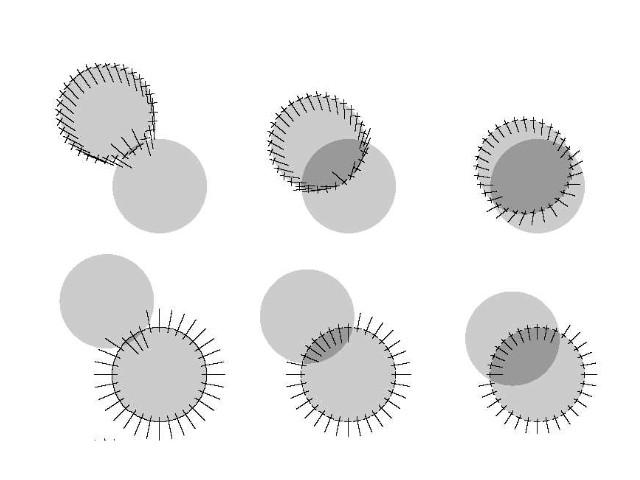
\includegraphics[width=1\textwidth]{figuras/demons.jpg}
    \caption{A primeira linha demonstra o sistema de atratores, enquanto a segunda o Demons, por \citep{thirion1995fast}}
    \label{fig:demons}
\end{figure}

\subsubsection{Aproximação matemática da transformação}
    O \textit{Demons} supõe que a transformação não muda a função de densidade, ou seja, ela só movimenta os pixels e não muda
suas intensidades. A equação seguinte resume isso:
\begin{align}
    i(x(t),y(t),z(t)) = const, \\
\end{align}
    onde $i$ é a intensidade da imagem na posição $x(t),y(t),z(t)$. Derivando (1) temos:
\begin{align}
    \frac{\partial i}{\partial x} \frac{\partial x}{\partial t} +
    \frac{\partial i}{\partial y} \frac{\partial y}{\partial t} = - \frac{\partial i}{\partial t}
\end{align}
    Supondo que as duas imagens que temos diferem de uma unidade de tempo $\partial i/\partial t = 
r-a$, \textit{r} e \textit{a} as intensidades de R e A respectivamente e que a velocidade instantânea 
$\vec{v} = (dx/dt,dy/dt)$ é aplicada a cada pixel para movê-lo de A para R, chegamos a equação:
\begin{align}
    \vec{v}*\vec{\nabla}r = a - r, \ \text{onde} \ \vec{\nabla} r \ \text{é o gradiente de R}
\end{align}
    O inverso da transformação é aproximado por $\vec{v}$. Porém essa equação é instável em relação a norma de $\nabla 
r$. Se a sua norma for muito pequena o \textit{Demon} em questão é levado para o infinito em alguma direção. Podemos levar em 
conta a diferença dos pixeis de R e A para normalizar a equação (4), obtendo a forma final do \textit{Demons}:
\begin{equation}
    \vec{v} = \frac{\vec{\nabla}r * (a - r)}{\vec{\nabla}r^2 * (a - r)^2}
\end{equation}

\subsubsection{Implementação}
    Como a formula (5) é degenerada, ou seja, não é possivel encontrar uma solução analiticamente para ela,
não podemos calcular o valor de $\vec{v}$ sem utilizar algum artificio. Para tal,
utilizaremos um algoritmo iterativo. Esse algoritmo recebe como entrada as imagens R e A e um campo vetorial
com as dimensões de A que contém uma aproximação da transformação aplicada, esse campo pode ser zero. 
Cada iteração realiza 3 passos:
\begin{enumerate}
    \item Para cada \textit{Demon} em $A_i$, calculamos $\vec{v_i}$, criando um novo campo vetorial $V_i$
    \item Aplicamos um filtro Gaussiano para retirar o ruído introduzido pelo processo em $V_i$
    \item Aplicamos $V_i$ em $A$ para obter $A_{i+1}$;
\end{enumerate}
    Esse processo é feito até que $A_i$ convirja à $R$. É importante lembrar que é necessário a
utilização de um algoritmo de interpolação, já que é extremamente provável que o vetor $\vec{v}$
leve os pontos para posições não inteiras. A interpolação trilinear já é suficiente para tal.

\subsubsection{\textit{Demons} Simétrico}\index{Demons Simétrico}
    O método acima é conhecido como \textit{Demons} Assimétrico, pois ele só utiliza informações vindas
da imagem referência. No mesmo artigo, Thirion propõe um outro método, conhecido como Simétrico.
Nele a equação para o cálculo de $\vec{v}$ leva o gradiente das imagens $A_i$. Ele obtém resultados
melhores ao custo do cálculo do gradiente de $A_i$ em toda iteração. Sua fórmula é dada por:
\begin{align}\label{math:demons}
    \vec{v} = \frac{4(a - r)*\vec{\nabla}r|\vec{\nabla}r||\vec{\nabla}a|}
                    {(\vec{\nabla}r+\vec{\nabla}a)^2*(\vec{\nabla}r^2 + \vec{\nabla}a^2 + 2(a - r)^2)}
\end{align}

\subsubsection{Pseudo Algoritmo e Tempo Assintotico de Execução do \textit{Demons} Simétrico}

  Abaixo temos a construção de um pseudo algoritmo do \textit{Demons} Simétrico, e de uma subfunção importante para sua 
execução, a \textit{calcularCampoInstantaneo}, que calcula o deslocamento dos \textit{Demons} na iteração atual, 
deslocamento esse que será somando ao campo de deslocamento total:

\begin{lstlisting}[mathescape]
demons(imagemReferencia, imagemAlvo, campoDeslocamento):
  gradienteRef <- calcularGradienteDaImagem(imagemReferencia)
  campoInstantaneo = 0
  execute:
    campoInstantaneoAntigo = campoInstantaneo
    imagemEstimada <- aplicarCampoAImagem(campoDeslocamento, imagemAlvo)
    campoInstantaneo <- calcularCampoInstantaneo(gradienteRef, imagemReferencia, imagemEstimada)
    campoInstantaneo = filtroGaussiano(campoInstantaneo)
    campoDeslocamento = campoDeslocamento + campoInstantaneo
  enquanto (campoInstantaneo - campoInstantaneoAntigo) <= $\epsilon$:
\end{lstlisting}

\begin{lstlisting}[mathescape]
calcularCampoInstantaneo(gradienteRef, imagemReferencia, imagemEstimada):
  campoInstantaneo = 0
  para x = 0, x menor que $n_l$ :
    para y = 0, y menor que $n_c$ :
      gradienteEstimado <- calcularGradienteDaImagem(imagemEstimada)
      diff = imagemEstimada[x,y] - imagemReferencia[x,y]
      vetorGradSimetrico = gradienteEstimado[x,y] + gradienteRef[x,y]
      campoInstantaneo[x,y] = $\frac{2*vetorGradSimetrico*diff}{(diff^2+vetorGradSimetrico^2)}$
  return campoInstantaneo
\end{lstlisting}

\begin{lstlisting}[mathescape]
calcularGradienteDaImagem(imagem):
  gradiente = 0
  para x = 0, x menor que $n_l$ :
    para y = 0, y menor que $n_c$ :
      gradienteLinha = $\frac{imagem[x+1,y] - imagem[x-1,y]}{2}$
      gradienteColuna = $\frac{imagem[x+1,y] - imagem[x-1,y]}{2}$
      gradiente[x,y] = {gradienteLinha, gradienteColuna}
  return gradiente
\end{lstlisting}

  As tabelas abaixo mostram o tempo de execução assintotico do \textit{Demons} Simétrico, totalizando 
$\mathcal{O}(x*n_l^2*n_c^2)$:

\begin{table}[H]
\begin{center}
\begin{tabular}{l|c}
\hline
Tempo de execução do algoritmo \textit{Demons} Simétrico \\
\hline
Linha&Tempo\\
\hline
2       &$\mathcal{O}(n_l*n_c)$ \\
3       &$\mathcal{O}(1)$\\
4       &$\mathcal{O}(1)$\\
5       &$\mathcal{O}(1)$\\
6       &$\mathcal{O}(n_l*n_c)$\\
7       &$\mathcal{O}(n_l^2*n_c^2)$\\
8       &$\mathcal{O}(n_l*n_c)$\\
9       &$\mathcal{O}(1)$\\
10       &$\mathcal{O}(x)$\\
\hline
Total   &$\mathcal{O}(x*n_l^2*n_c^2)$\\
\hline
\end{tabular}
\caption{Tempo de execução do algoritmo \textit{Demons} Simétrico}
\label{table:tps}
\end{center}
\end{table}

\begin{table}[H]
\begin{center}
\begin{tabular}{l|c}
\hline
Tempo de execução do algoritmo \textit{calcularCampoInstantaneo} \\
\hline
Linha&Tempo\\
\hline
2       &$\mathcal{O}(1)$ \\
3       &$\mathcal{O}(n_l)$ \\
4       &$\mathcal{O}(n_c)$\\
5       &$\mathcal{O}(n_l*n_c)$\\
6       &$\mathcal{O}(1)$\\
7       &$\mathcal{O}(1)$\\
8       &$\mathcal{O}(1)$\\
9       &$\mathcal{O}(1)$\\
\hline
Total   &$\mathcal{O}(n_l^2*n_c^2)$\\
\hline
\end{tabular}
\caption{Tempo de execução do algoritmo \textit{calcularCampoInstantaneo}}
\label{table:interpolar}
\end{center}
\end{table}

\begin{table}[H]
\begin{center}
\begin{tabular}{l|c}
\hline
Tempo de execução do algoritmo \textit{calcularGradienteDaImagem} \\
\hline
Linha&Tempo\\
\hline
2       &$\mathcal{O}(1)$ \\
3       &$\mathcal{O}(n_l)$ \\
4       &$\mathcal{O}(n_c)$\\
5       &$\mathcal{O}(1)$\\
6       &$\mathcal{O}(1)$\\
7       &$\mathcal{O}(1)$\\
8       &$\mathcal{O}(1)$\\
\hline
Total   &$\mathcal{O}(n_l*n_c)$\\
\hline
\end{tabular}
\caption{Tempo de execução do algoritmo \textit{calcularGradienteDaImagem}}
\label{table:interpolar}
\end{center}
\end{table}

\subsubsection{Aceleração do \textit{Demons}}
    O primeiro passo do algoritmo iterativo pode ser acelerado utilizando a arquitetura SIMD. O calculo de um dos vetores
depende do gradiente $\vec{\nabla}r$ e da diferença entre as intensidades da imagem Alvo e Referência $(a - r)$, logo
todos os passos podem ser realizados em paralelo sem perda de desempenho. Tanto a aplicação do filtro gaussiano como
a aplicação do campot vetorial $V$ também podem ser adaptados para a SIMD, pelo mesmo motivo apresentado anteriormente.
Devemos tomar cuidado para garantir que os passos sejam executadas de forma sequencial, ou seja, nenhum pixel deve começar
a execução do passo 2 antes que todos tenham executado o passo 1.

%% ------------------------------------------------------------------------- %%
\subsection{Thin Plate Splines}\index{TPS}
    O Thin Plate Splines (TPS) segue mais à risca os passos gerais de um algoritmo de registro. Ele utiliza
características para criar uma função de interpolação que é utilizada para criar a imagem registrada a partir
da imagem referência. Vários algoritmos podem ser utilizados para adquirir as características que serão usadas
pelo TPS, mas não abordaremos esse assunto pois ele foge do escopo do trabalho. Assumimos no inicio da sua
execução que 2 conjuntos de características existem, um para cada imagem, e que uma correspondência entre
eles já é estabelecida.

    Dados as características na imagem referência $(x_i,y_i, i=1,..,n)$ e na imagem alvo $(X_i,Y_i, i=1,..,n)$
o TPS cria uma função que mapeia exatamente cada característica da imagem referência na sua
correspondente na imagem alvo e que é capaz de interpolar os pontos restantes para a imagem final. Para realizar
essa tarefa é utilizada uma função que define uma superfície que sofre a ação de pesos centrados nas
características da imagem referência. A superfície é definida pela seguinte equação, escrita por \cite{bookstein1989principal}:

\begin{align}\label{math:tps}
    f(x,y) = A_0 + A_1x + A_2y + \sum_{i=0}^n F_i r_i^2 ln r_i^2
\end{align}
Onde $r_i^2 = (x-x_i)^2 + (y-y_i)^2 + d^2$, $d$ é um fator de rigidez da superfície, quanto mais próximo de 
zero $d$ é mais a superfície sofre ação dos pontos de controle, e os pontos $(x_i, y_i)$ são os pontos de controle.

    O TPS deve então determinar os valores das variáveis $A_0, A_1, A_2$ e dos $F_i$. 
Isso é feito através do sistema linear:

\begin{align}
\begin{split}
    \sum_{i=1}^n F_i &= 0 \\
    \sum_{i=1}^n F_ix &= 0 \\
    \sum_{i=1}^n F_iy &= 0 \\
    f(x_1,y_1) &= A_0 + A_1x + A_2y + \sum_{i=0}^n F_i r_{i1}^2 ln r_{i1}^2 \\
    \vdots \\
    f(x_n,y_n) &= A_0 + A_1x + A_2y + \sum_{i=0}^n F_i r_{in}^2 ln r_{in}^2
\end{split}
\end{align}

A equação $\sum_{i=1}^n F_i = 0$ faz com que a soma dos pesos aplicados a superfície seja zero, fazendo com que
ele não se mova. As equações $\sum_{i=1}^n F_ix = 0$ e $\sum_{i=1}^n F_iy = 0$ garantem que a superfície não vai girar.

    Esse sistema deve ser resolvido duas vezes, uma para $f(x,y) = X$ e outra para $g(x,y) = Y$. Com todas as variáveis
encontradas, podemos aplicar as funções de interpolação para desenhar a imagem final.

\subsubsection{Pseudo Algoritmo e Tempo Assintotico de Execução}

  Abaixo temos a construção de um pseudo algoritmo do tps, e de uma subfunção importante para sua execução, a 
\textit{interpolar}, que realiza a interpolação da imagem Alvo na construção da imagem registrada:

\begin{lstlisting}[mathescape]
tps(imagemReferencia, imagemAlvo, caracImagemRef, caracImagemAlvo):
  solucaoDaEquLinearEmX <- resolverEquLinear(caracImagemRef, caracImagemAlvo)
  solucaoDaEquLinearEmY <- resolverEquLinear(caracImagemRef, caracImagemAlvo)
  para x = 0, x menor que $n_l$ :
    para y = 0, y menor que $n_c$ :
      novoPontoX <- interpolar(x,y, solucaoDaEquLinearEmX, caracImagemRef)
      novoPontoY <- interpolar(x,y, solucaoDaEquLinearEmY, caracImagemRef)
      novaImagem[x, y] = imagemAlvo[novoPontoX, novoPontoY]
\end{lstlisting}

\begin{lstlisting}[mathescape]
interpolar(x, y, solucaoDaEquLinear, caracImagemRef):
  v[0] = 1
  v[1] = x
  v[2] = y
  para n = 0, n menor que $n_{cp}$ :
    xi = caracImagemRef[n].x
    yi = caracImagemRef[n].y
    r = $\sqrt{(x-xi)^2 + (y-yi)^2}$
    v[n+3] = $r*\log{r}$
  return $v \cdot solucaoDaEquLinear$ 
\end{lstlisting}

  As tabelas abaixo mostram o tempo de execução assintotico do tps, totalizando 
$\mathcal{O}(\frac{4}{3}n_{cp}^3+n_l*n_c*n_{cp})$:

\begin{table}[H]
\begin{center}
\begin{tabular}{l|c}
\hline
Tempo de execução do algoritmo \textit{tps} \\
\hline
Linha&Tempo\\
\hline
2       &$\mathcal{O}(\frac{2}{3}n_{cp}^3)$\\
3       &$\mathcal{O}(\frac{2}{3}n_{cp}^3)$\\
4       &$\mathcal{O}(n_l)$\\
5       &$\mathcal{O}(n_c)$\\
6       &$\mathcal{O}(n_{cp})$\\
7       &$\mathcal{O}(n_{cp})$\\
8       &$\mathcal{O}(1)$\\
\hline
Total   &$\mathcal{O}(\frac{4}{3}n_{cp}^3+n_l*n_c*n_{cp})$\\
\hline
\end{tabular}
\caption{Tempo de execução do algoritmo \textit{tps}}
\label{table:tps}
\end{center}
\end{table}

  O tempo de execução da resolução do sistema linear foi retirada do livro escrito por 
\cite[Part~IV]{trefethen1997numerical}, assumindo uma fatoração LU da matriz.

\begin{table}[H]
\begin{center}
\begin{tabular}{l|c}
\hline
Tempo de execução do algoritmo \textit{interpolar} \\
\hline
Linha&Tempo\\
\hline
2       &$\mathcal{O}(1)$ \\
3       &$\mathcal{O}(1)$ \\
4       &$\mathcal{O}(1)$\\
5       &$\mathcal{O}(n_{cp})$\\
6       &$\mathcal{O}(1)$\\
7       &$\mathcal{O}(1)$\\
8       &$\mathcal{O}(1)$\\
9       &$\mathcal{O}(1)$\\
10      &$\mathcal{O}(n_{cp}+3)$\\
\hline
Total   &$\mathcal{O}(n_{cp})$\\
\hline
\end{tabular}
\caption{Tempo de execução do algoritmo \textit{interpolar}}
\label{table:interpolar}
\end{center}
\end{table}

\subsubsection{Aceleração do Thin Plate Splines}

    O primeiro passo para acelerar o TPS é utilizar algoritmos para resolver o sistema linear diretamente na GPU, o que
não é dificil dado que a matriz que representa o sistema sempre é simetrica com uma diagonal de zeros por construção. O
próximo passo para realizar a acelereção do TPS é criar dois vetores que guardam todos os valores possíveis de $(x-x^i)^2$
e $(y-y^i)^2$. O uso desses vetores diminui o número de operações necessárias de $n_l*n_c*n_{cp}$ para $(n_l+n_c)*n_{cp}$.
Da maneira original, a operação $(x-x^i)^2$ é repetida $n_c$ vezes para cada coluna, já com o uso dos vetores esse valor
é calculado uma única vez e acessado toda vez que ele é necessário.


% Colocar outros algoritmos de regitro %         % associado ao arquivo: 'cap-conceitos.tex'
%% ------------------------------------------------------------------------- %%
\chapter{Metodologia}
\label{cap:metodologia}

%% ------------------------------------------------------------------------- %%
\section{Mapeamento do Thin Plate Splines para GPU}

  O TPS é composto de dois passos, como descrito na seção \ref{thinPlateSplines}.
No primeiro passo, um sistema linear é construido usando os pares de correspondências
encontradas nas duas imagens de entrada, e resolvido afim de encontrar os parâmetros
da função de deformação. O próximo passo é o calculo da função de deformação em
todos os pontos da imagem alvo, gerando a imagem resultado.

\subsection{Mapeamento da resolução do sistema linear}

  Pela natureza da sua construção, os sistemas lineares montados pelos TPS dificilmente
serão esparsos, logo algoritmos mais simples podem ser aplicados na sua solução
sem perda de desempenho. Essa etapa de mapeamento foi resolvida escolhendo a
biblioteca \textit{cuSolver}, da \cite{cuSolver}. A fatoração QR foi escolhida
para resolver o sistema linear.

  Os sistemas lineares tem tamanho $n_{cp}^2$, e a solução tem tamanho $n_{cp}$.
Logo, é necessário transferir $(n_{cp}^2 + n_{cp}) \times 3 \times 8$ bytes de
dados para a GPU. O \textit{cuSolver} utiliza a matriz com o sistema linear para
armazenar os resultados dos passos intermediários, deminuindo o consumo de memória
do algoritmo.

\subsection{Mapeamento da função de deformação}\label{segundoPasso}

  O segundo passo do TPS envolve a função de deformação e a interpolação dos
resultados da mesma. Como entrada são recebidos os resultados do passo anterior,
os voxels da imagem alvo e a lista das características. O resultado final é gravado
em memória da GPU, que é copiado para a memória da CPU após a execução do kernel.

  O passo foi implementado em um kernel CUDA na linguagem C. Cada thread do Kernel
é mapeada para o cálculo da função de deformação de um voxel da imagem, logo são necessários
$\left \lceil{\frac{n_l}{8}}\right \rceil \times
\left \lceil{\frac{n_c}{8}}\right \rceil \times
\left \lceil{\frac{n_p}{8}}\right \rceil$ blocos, respectivamente para
cada dimensão da image, e cada bloco tem dimensão $8 \times 8 \times 8$.

  Somando o espaço em memória dos parametros com o da imagem resultado, o kernel
reserva $N \times 2 \times 1 + n_{cp} \times 6 \times 8$ bytes

  Com os resultados em mãos, o segundo passo é calcular a função de deformação.
A função foi implementada em um kernel CUDA. É necessário prover os voxels da
imagem alvo, as soluções dos três sistemas lineares, a lista de pontos de controle
e o espaço em memória para gravar a imagem resultado. São necessários, então,
$(N \times 2 + n_{cp} \times 6) \times 8$ bytes. O código do kernel é:

\begin{lstlisting}
  __global__ void tpsCuda(short* cudaImage, short* cudaRegImage,
                          float* solutionX, float* solutionY,
                          float* solutionZ, int width, int height,
                          int slices, float* keyX, float* keyY,
                          float* keyZ, int numOfKeys) {
    int x = blockDim.x*blockIdx.x + threadIdx.x;
    int y = blockDim.y*blockIdx.y + threadIdx.y;
    int z = blockDim.z*blockIdx.z + threadIdx.z;

    float newX = solutionX[0]+x*solutionX[1]+y*solutionX[2]+z*solutionX[3];
    float newY = solutionY[0]+x*solutionY[1]+y*solutionY[2]+z*solutionY[3];
    float newZ = solutionZ[0]+x*solutionZ[1]+y*solutionZ[2]+z*solutionZ[3];

    for (int i = 0; i < numOfKeys; i++) {
      float r = (x-keyX[i])*(x-keyX[i])+  (y-keyY[i])*(y-keyY[i])+(z-keyZ[i])*(z-keyZ[i]);
      if (r != 0.0) {
        newX += r*log(r)*solutionX[i+4];
        newY += r*log(r)*solutionY[i+4];
        newZ += r*log(r)*solutionZ[i+4];
      }
    }

    if (x <= width-1 && x >= 0)
      if (y <= height-1 && y >= 0)
        if (z <= slices-1 && z >= 0)
          cudaRegImage[z*height*width+y*width+x] = cudaTrilinearInterpolation(newX, newY, newZ, cudaImage, width, height, slices);
  }
\end{lstlisting}

  As linhas 6, 7 e 8 usam o ID do bloco e ID da thread para calcular o voxel que será
gerado. As linhas 10, 11 e 12 cálculam a deformação rígida. O laço da linha 14
cálcula da deformação não-rigida. Por fim, uma interpolação trilinear é aplicada
para resgatar a intensidade do voxel da imagem alvo que é usada para gerar a image
resultado. A checagem antes da interpolação é necessária pois o número de threads
usadas pelo kernel é maior que o número de voxels da imagem, salvo pelas dimensões
que sejam multiplas de 8.

  TODO: FAZER A IMAGEM DE MAPEAMENTO DAS THREADS PARA VOXELS.

%% ------------------------------------------------------------------------- %%
%% ------------------------------------------------------------------------- %%
\section{Melhorias de desempenho}

  O objetivo desse trabalho é apresentar uma implementação de alto desempenho
do algoritmo Thin plate splines em um ambiente GPGPU. O mapeamento apresentado
na seção anterior, por maior que seja seu aumento de velocidade comparativamente
com uma implementação em CPU, não utiliza nenhum método de melhoria de desempenho.
Essa seção se aprofunda em métodos aplicados para o aumento do desempenho de
algoritmos desenvolvidos em \textbf{CUDA}, enquanto avaliamos a aplicabilidade
de táis métodos ao TPS.

\subsection{Melhorias de desempenho associadas à memória}

O acesso a memória é o responsável por grande parte da queda de desempenho
em kernels. Isso se deve, em grande parte, pela diferença de comunicação entre o
\textit{Host} e a memória principal da GPU e a comunicação entre a memória
principal da GPU e os multiprocessadores
(8 GB/s contra 177.6 GB/s na comparação feita em \cite{cudaBestPractices}). Logo,
a transferência de memória entre \textit{Host} e \textit{Device} deve ser
minimizada. Para tanto, a implementação apresentada neste trabalho realiza uma
etapa de pré-processamento onde o máximo de memória é reservado na GPU.

A implementação é focada no registro de várias imagens alvo para uma única
imagem referência, logo os dados da imagem referência são transmitidos para a
GPU uma única vez. O TPS só utiliza a lista de características da imagem referência.
O próximo passo é ocupar o máximo possível de memória com instâncias diferentes
de registro. Cada instância de registro, como dito na seção \ref{segundoPasso},
precisa dos voxels da imagem alvo, das suas características e de espaço suficiente
para guardar a imagem resultado. Ainda para diminuir o tempo de transferência,
as soluções dos sistemas lineares são mantidos em memória na GPU.

O segundo método utilizado foi o mapeamento dos voxels da imagem alvo para uma
textura tridimensional. A memória de textura é preservada em cache, com privilégio
somente de leitura. Além disso, estão presentes no hardware as seguintes operações
em texturas: interpolação, normalização de coordenadas e checagem automática de
fronteira.

Por último, a fim de minimizar o \textit{downtime} dos multiprocessadores da GPU, a
execução paralela de várias instâncias de registro foi aplicada. O paralelismo
é iniciado na CPU, onde cada chamada do kernel do TPS parte de uma thread separada.
O escalonador da GPU é capaz de criar contextos diferentes para cada instância
diferente, e organizar os recursos da GPU entre todas as instâncias. A execução
em paralelo de vários kernels esconde a latência de cópia de memória entre a
CPU e GPU executando um kernel que já esteja pronto enquanto popula a memória
para a execução de outro.

No entanto, nem todas as técnicas de melhoria de desempenho são aplicáveis ao
TPS. O uso de \textit{Pinned memory}, método em que a memória da CPU é mapeada
diretamente a uma região da memória da CPU, aumentando a taxa de transferência entre
os diferentes espaços de memória. Mas esse mapeamento introduz uma restrição ao
kernel, já que leituras ou escritas feitas por threads diferentes ao mesmo banco
de memória causam lentidão. A memória compartilhada não foi explorada, já que
cada bloco divide entre todas as suas \textit{threads} uma pequena seção do
bloco de memória compartilhada, o que limita o que pode ser mantido nesta região.

\subsection{Melhorias de desempenho associadas ao processamento}

  Melhorar o desempenho do processamento de um kernel quer dizer maximizar o
tempo que cada um dos multiprocessadores está ocupando executando algo. Atingir
esse objetivo não é trivial, pois a distribuição das threads entre multiprocessadores
é parametrizada por vários fatores como o número disponível de registradores
em cada multiprocessador e a quantidade de memória compartilhada por bloco, por exemplo.
Como explicado na seção \ref{GPU}, o warp é a menor unidade de execução em um
multiprocessador. Cada warp é constituída de 32 \textit{threads}, que executam,
ao mesmo tempo, a mesma linha de código. A razão entre o número máximo de warps
em execução de um kernel pelo número máximo de warps em execução no hardware,
chamada de \textbf{Ocupação}, será a métrica usada para calcular o desempenho
de um kernel.

  A API do CUDA disponibiliza uma função que recebe o kernel e um tamanho de
bloco e retorna a ocupação da GPU dado esses parametros. Utilizando essa função,
uma calculadora de Ocupação foi construida. A calculadora incrementa o
tamanho do bloco de 32 em 32 threads (para garantir que um novo warp sempre
seja criado), e o bloco que obter a maior taxa de Ocupação é escolhido, com
preferência para blocos pequenos se houver algum empate. Essa preferência beneficia
a execução em paralelo de vários kernels.

  Outra técnica aplicada foi a de controlar o número de registradores do kernel.
Sejam $TM$ o número máximo de \textit{threads} por multiprocessador e $RB$ o
número máximo de registradores por bloco, o número máximo de registradores que
cada \textit{thread} pode usar é $\left \lceil{\frac{RB}{TM}}\right \rceil$.
O número de registradores utilizado por thread pode ser verificado pelas flags
de compilação \textit{-Xptxas -v}. Nas arquiteturas atuais, o número de
registradores deve ficar abaixo de $32$ por thread. Esse número foi atingido pelos
kernels escritos para este trabalho.

  Maximizar o número de \textit{threads} executando em um dado momento ajuda em
esconder a latência das instruções das mesmas. Ao executar uma instrução,
como por exemplo um acesso a memória, todas as \textit{threads} de um warp
ficam bloqueadas esperando o resultado. Para compensar isso, o multiprocessador
pode executar instruções de um outro warp. Como definido em \cite{cudaProgrammingGuide},
seja $L$ a quantidade de ciclos do \textit{clock} necessário para executar uma
instrução, são necessárias $8L$ instruções para esconder sua latência, dado um
\textit{device} de \textit{compute capabillity} $3.x$.

  Por fim, a execução paralela de vários kernels, alem de esconder a latência
na cópia de memória como dito na seção acima, esconde a latência de instruções.
Com vários kernels executando ao mesmo tempo, o escalonador da GPU pode escolher
um warp associado a outro kernel enquanto espera a execução de outro warp.
         % associado ao arquivo: 'cap-conceitos.tex'
%% ------------------------------------------------------------------------- %%
\chapter{Resultados}
\label{cap:resultados}

%% ------------------------------------------------------------------------- %%
%% ------------------------------------------------------------------------- %%
\section{Experimentos}
  Os testes foram inspirados pelo estudo de \cite{zagorchev2006comparative}.
A imagem Referência utilizada para os testes foi retirada do software BioImage
\cite{papademetris2005bioimage}, uma ressonância magnética cerebral. A imagem
alvo foi construida aplicando uma função senoidal com diferentes parâmetros
nas três dimensões da imagem referência. A função de deformação escolhida foi:

\begin{align} \label{math:composta}
\begin{split}
  X &= x + 2*sin(\frac{y}{8}) - 2*cos(\frac{z}{16}) \\
  Y &= y + 4*sin(\frac{x}{8}) - 2*sin(\frac{z}{8}) \\
  Z &= z + 2*sin(\frac{x}{16}) - 4*cos(\frac{y}{8})
\end{split}
\end{align}

\begin{figure}[H]
    \centering
    \begin{subfigure}[t]{0.8\textwidth}
      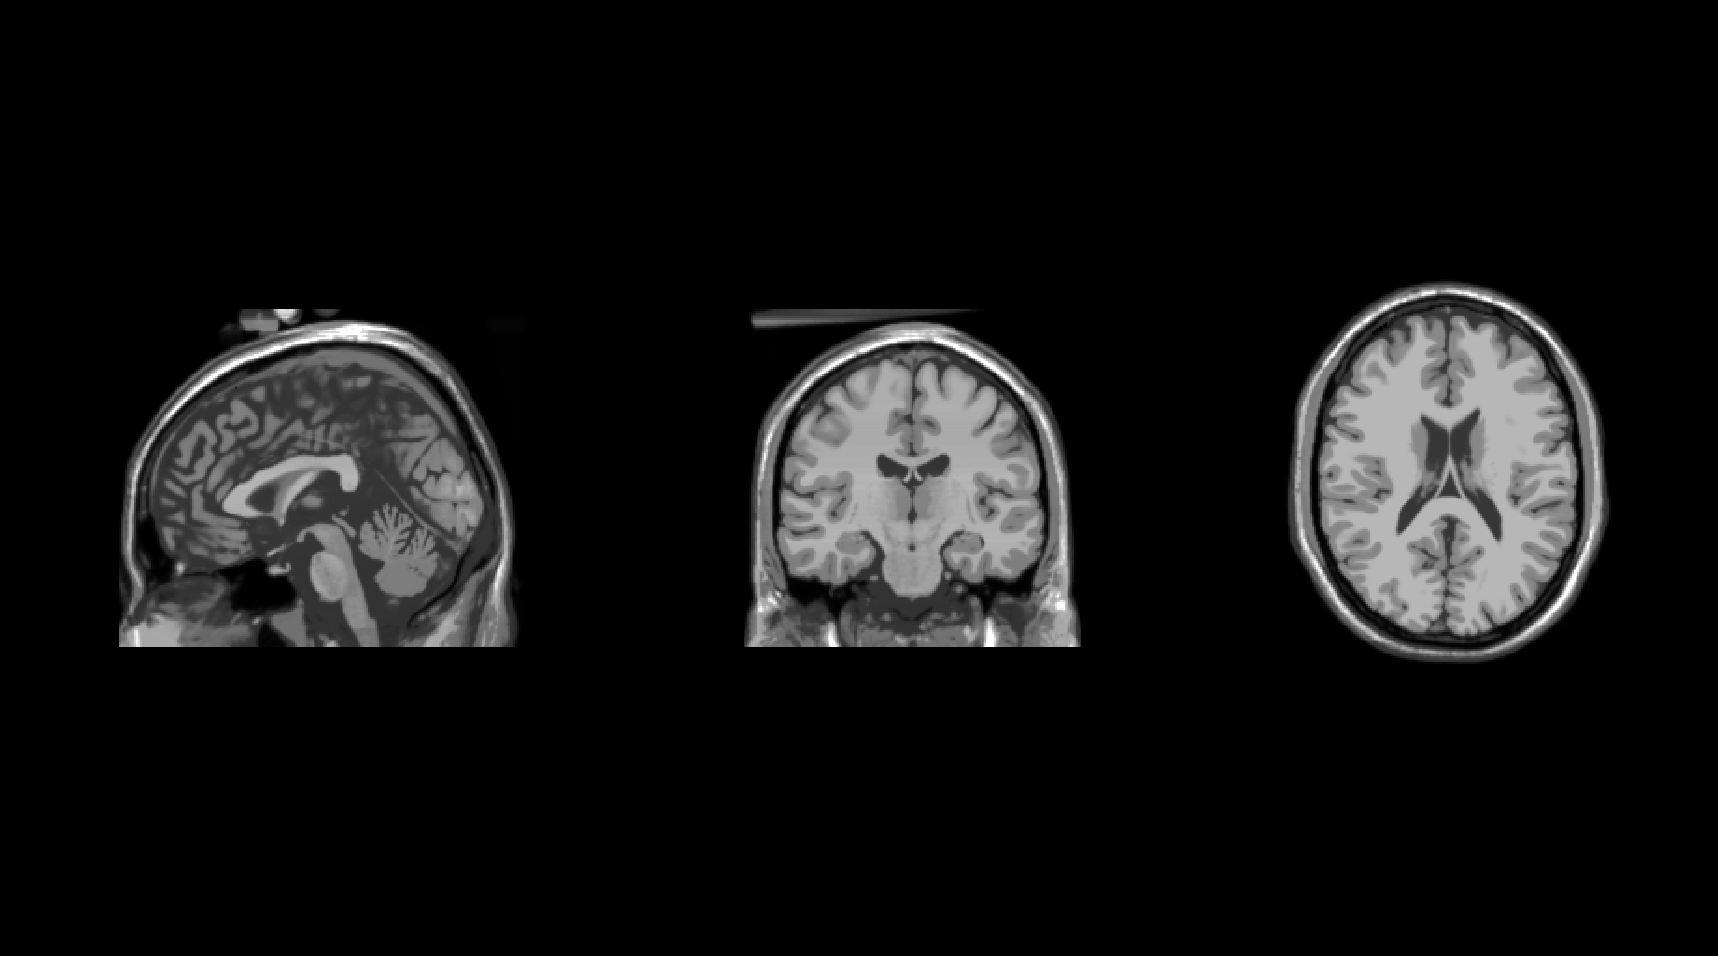
\includegraphics[width=\textwidth]{figuras/referenceImg.png}
      \subcaption*{(a)}
      \label{fig:unequalizedImage}
    \end{subfigure}
    \begin{subfigure}[t]{0.8\textwidth}
      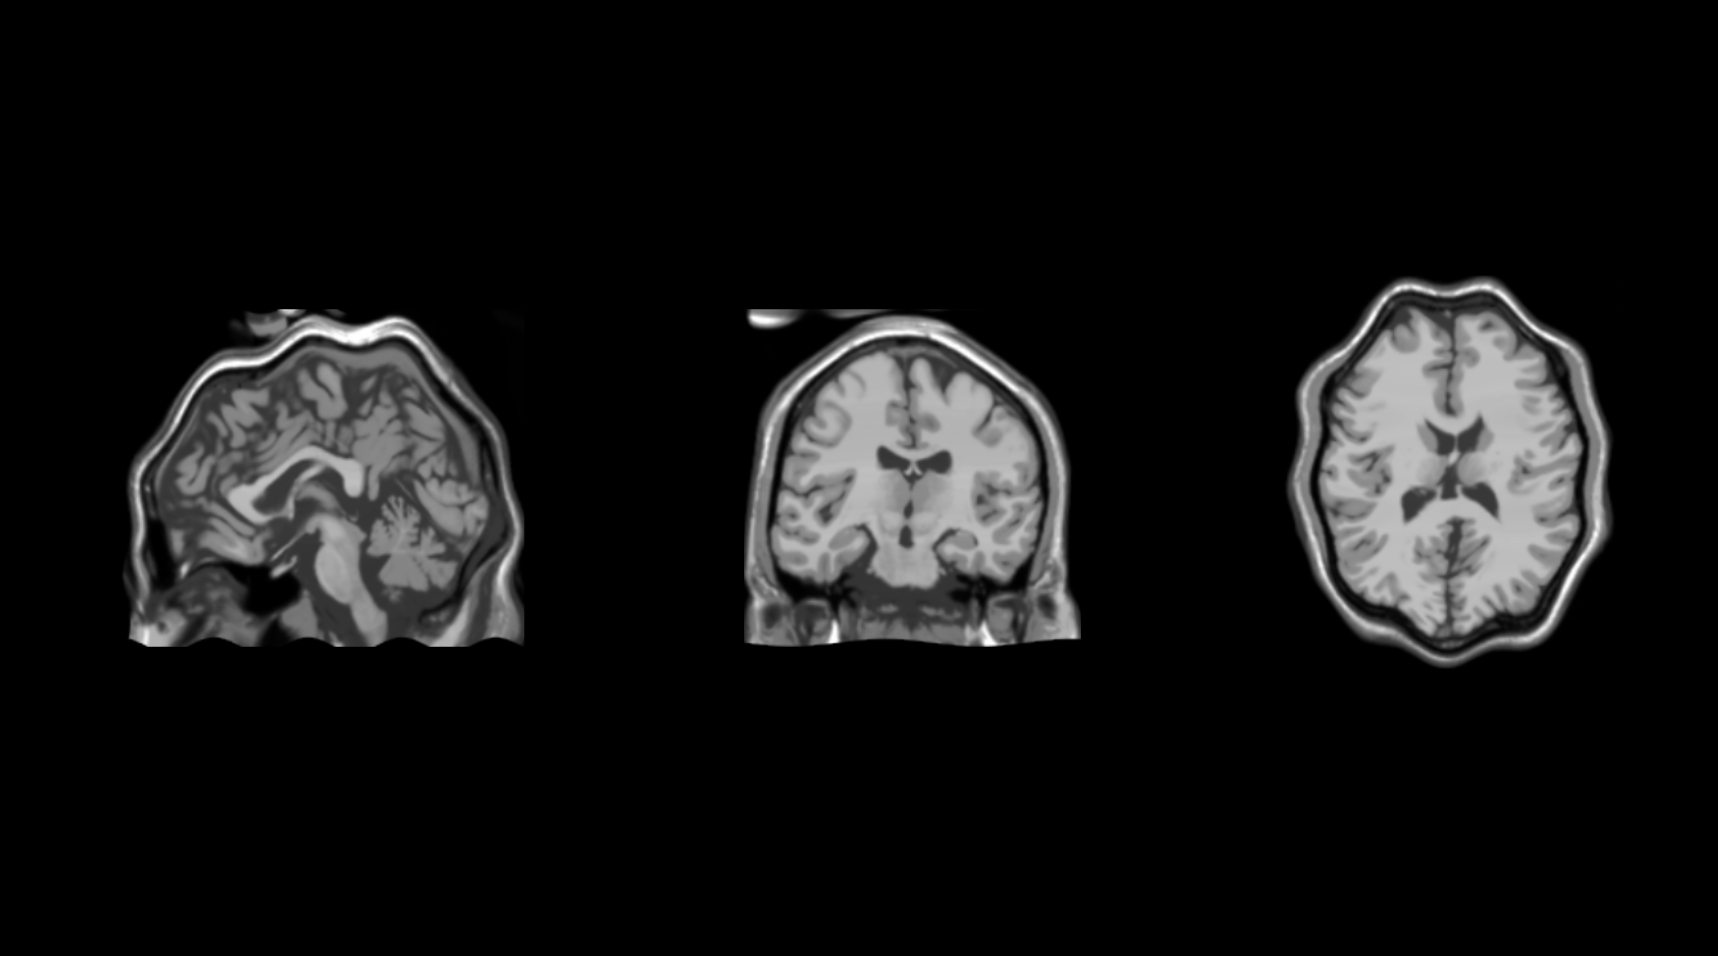
\includegraphics[width=\textwidth]{figuras/targetImg.png}
      \subcaption*{(b)}
      \label{fig:equalizedImage}
    \end{subfigure}
    \source{\cite{papademetris2005bioimage}}
    \caption{Imagens usadas nos testes. A primeira coluna é um corte sagital,
             a segunda coluna um corte coronal e a última um corte axial.
             (a) Imagem referência. (b) Imagem alvo.}
    \label{fig:equalization}
\end{figure}

  A construção artificial das imagens alvo foi escolhida pelos seguintes motivos:
(1) provar a aplicabilidade do algoritmo TPS não é nosso objetivo, (2) com a
função que provocou a deformação em mãos, gerar um conjunto de características
se torna um processo trivial, assim como encontrar as correspondências entre
elas, e (3) a corretude da nossa implementação do TPS é facilmente verificavel.

  Para apurar o ganho de desempenho de cada uma das possiveis modificações
descritas na seção \ref{melhoriaDesempenho}, elas foram implementadas de tal
maneira que elas podem ser ativadas ou desativadas independentemente atráves de
um arquivo de configuração. Logo, nosso casos de teste são:

\begin{enumerate}
  \item Paralelamente em CPU (nosso \textit{guideline})
  \item GPU sem nenhuma das melhorias ativadas
  \item Melhoria de cálculo de Ocupação
  \item Melhoria de textura 3D
  \item Melhoria de execução em paralelo
  \item Todas as combinações de duas melhorias ativas por vez
  \item Todas as melhorias ativas
\end{enumerate}

  Cada teste é composto de quatro execuções do TPS, registrando a mesma imagem
alvo com a mesma imagem referência. As características da imagem referência
são distribuidas uniformemente pelas dimensões da imagem, com um fator que
determina a quantidade de características utilizadas. As características da
imagem alvo são construidas aplicando a função de deformação em cada uma das
características da imagem referência, criando um cenário ideal para a execução
do TPS.

  Os testes foram executados em duas máquinas. A primeira é um notebook com
um processador quadcore Intel i5-3337U @ 1.80GHZ, 6GB de memória, e uma GPU
NVIDIA GeForce GT 730M com 384 cuda cores divididos em 2 multiprocessadores e
2GB de memória dedicada. A segunda máquina é uma máquina virtual, com 4
processadores de 2.3GHz, 8GB de memória, e uma GPU GeForce GTX 980 com 2048
cuda cores divididos em 16 multiprocessadores e 4GB de memória dedicada.

\begin{figure}[H]
    \centering
    \begin{subfigure}[t]{0.5\textwidth}
      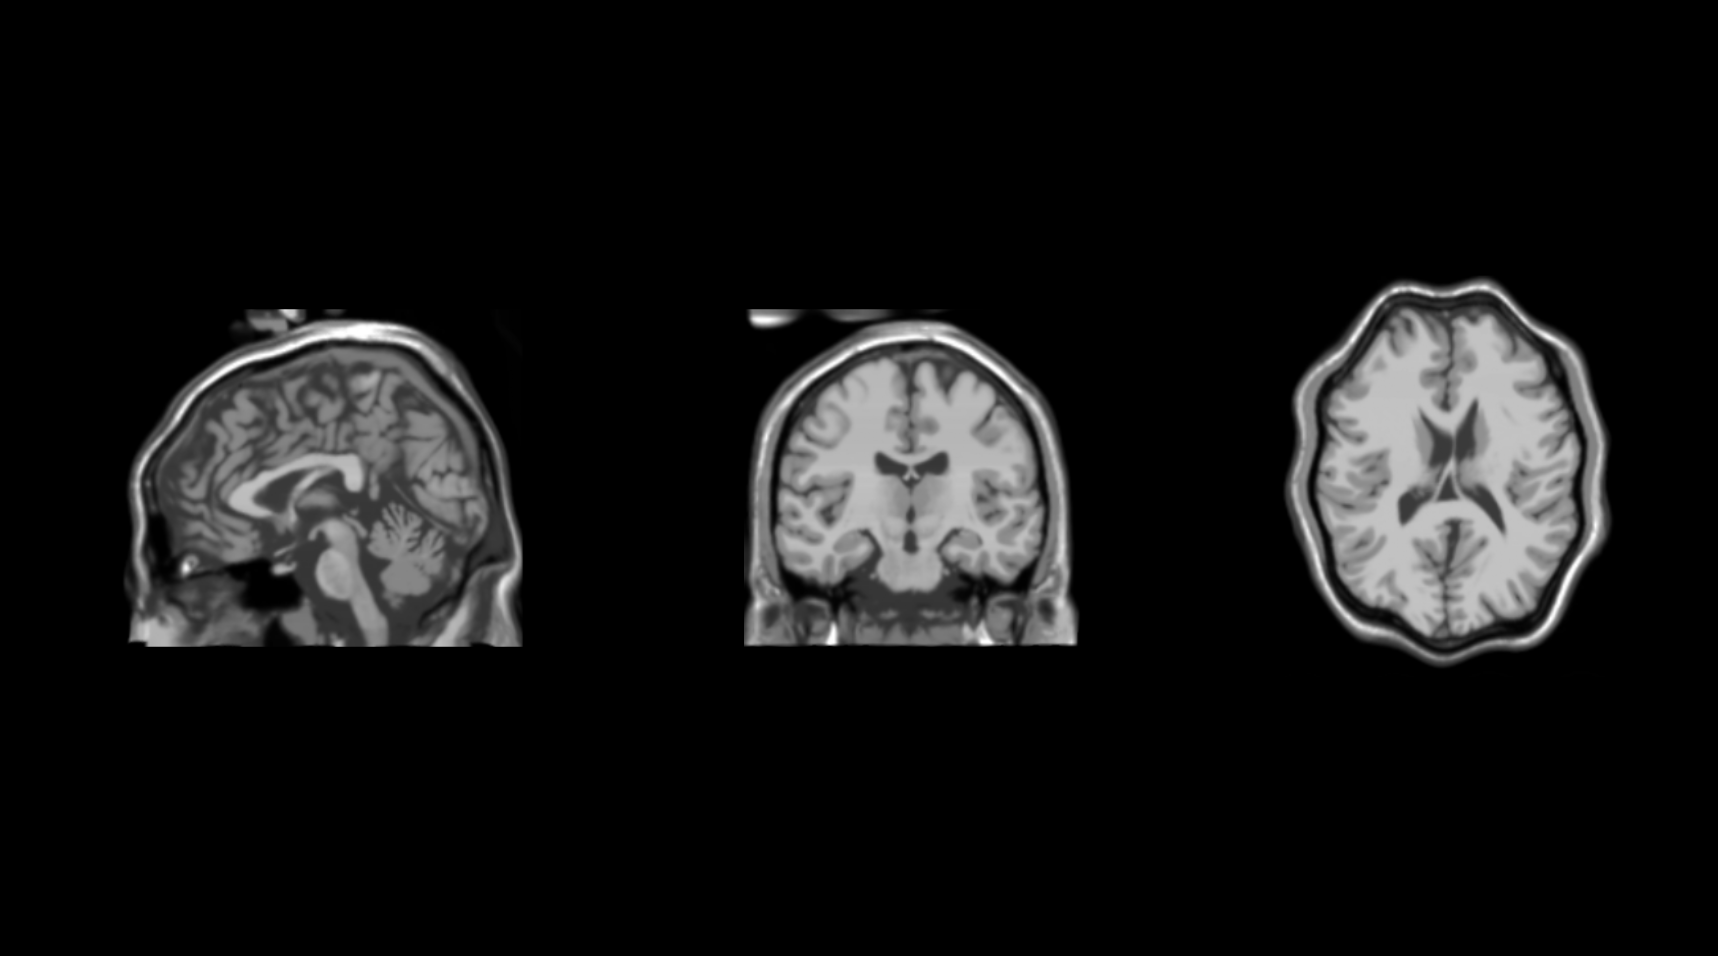
\includegraphics[width=\textwidth]{figuras/result001.png}
      \subcaption*{(a)}
      \label{fig:unequalizedImage}
    \end{subfigure}
    \begin{subfigure}[t]{0.5\textwidth}
      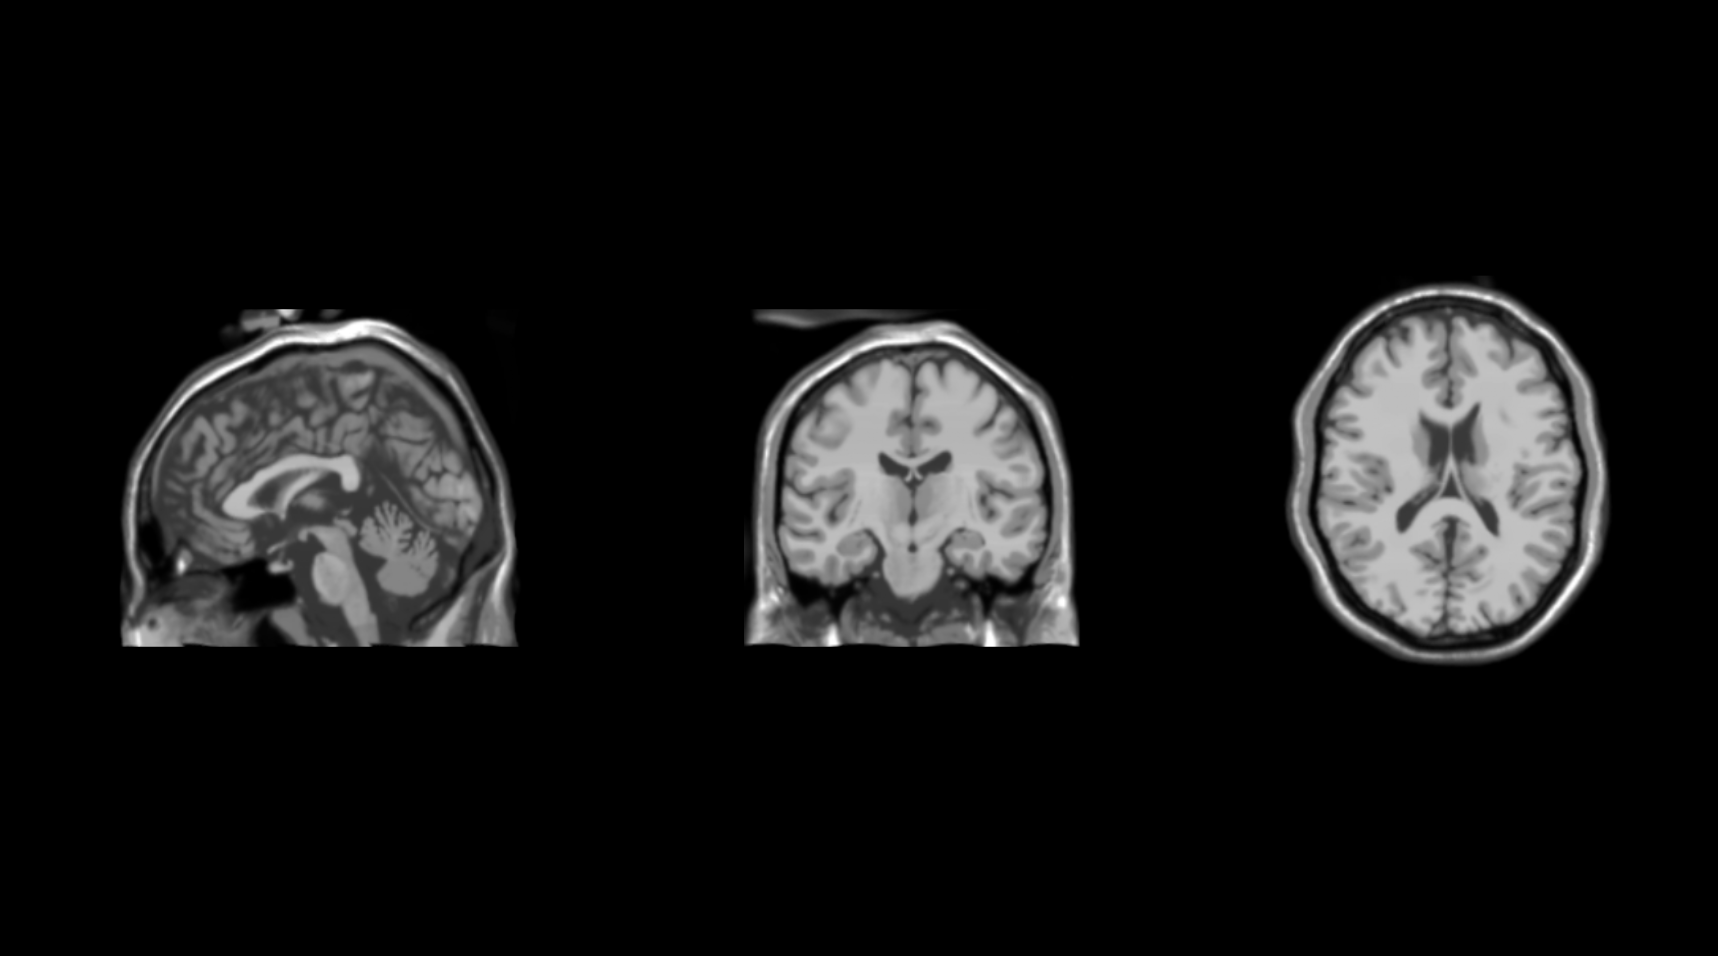
\includegraphics[width=\textwidth]{figuras/result002.png}
      \subcaption*{(b)}
      \label{fig:equalizedImage}
    \end{subfigure}
    \begin{subfigure}[t]{0.5\textwidth}
      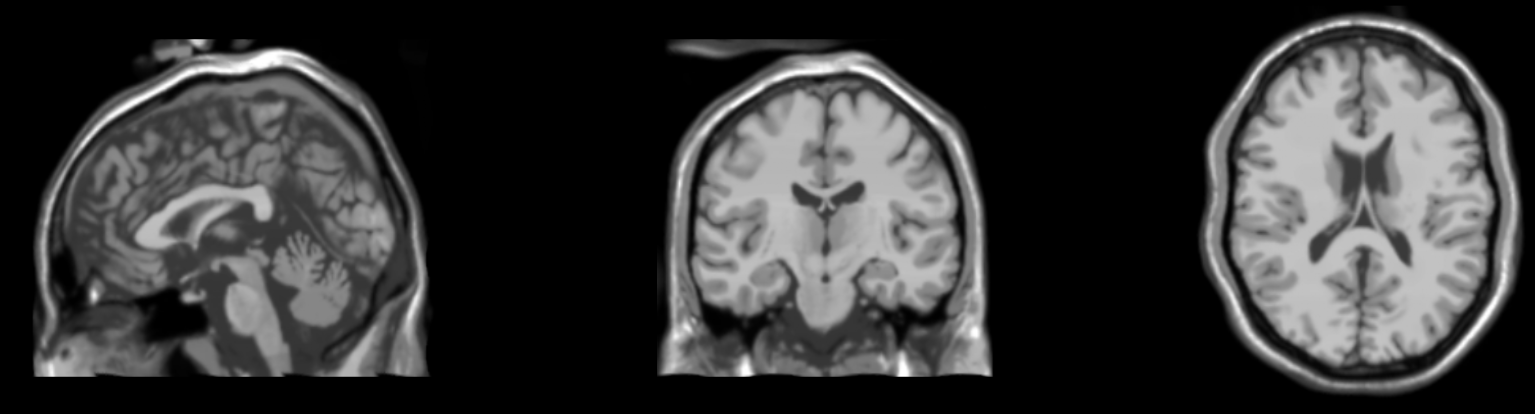
\includegraphics[width=\textwidth]{figuras/result003.png}
      \subcaption*{(c)}
      \label{fig:equalizedImage}
    \end{subfigure}
    \begin{subfigure}[t]{0.5\textwidth}
      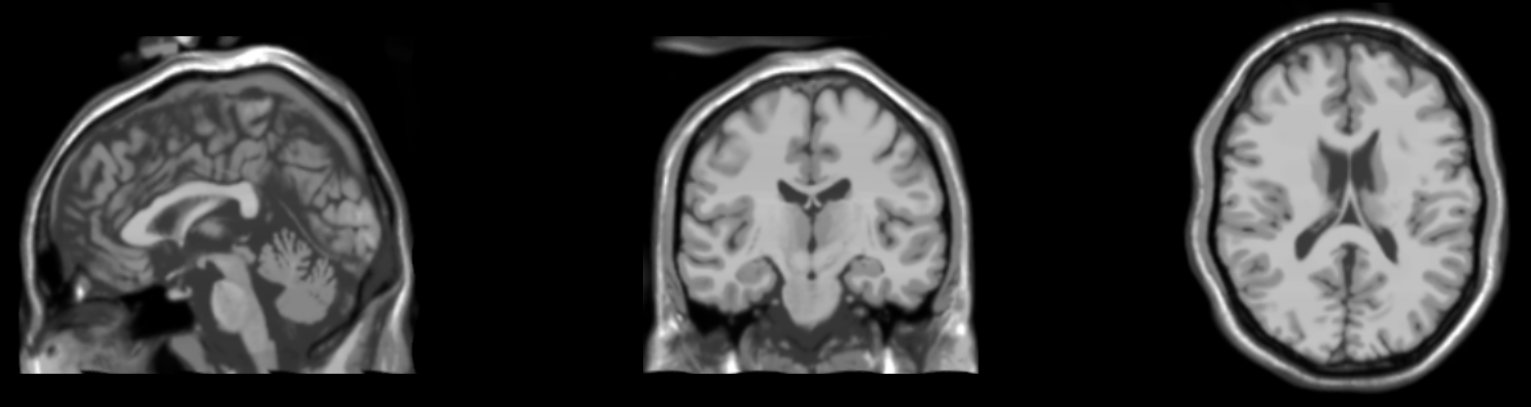
\includegraphics[width=\textwidth]{figuras/result004.png}
      \subcaption*{(d)}
      \label{fig:equalizedImage}
    \end{subfigure}
    \caption{Resultado dos testes. A primeira coluna é um corte sagital,
             a segunda coluna um corte coronal e a última um corte axial.
             (a) Resultado utilizando 576 características.
             (b) Resultado utilizando 2016 características.
             (c) Resultado utilizando 4864 características.
             (d) Resultado utilizando 7942 características.}
    \label{fig:equalization}
\end{figure}
        % associado ao arquivo: 'cap-resultados.tex'
% %% ------------------------------------------------------------------------- %%
\chapter{Proposta}
\label{cap:conclusoes}

	O aumento da qualidade de imagens proveniente da melhoria da tecnologia associada com câmeras e afins, juntamente com
a crescente facilidade de manter e utilizar grande quantidade de dados melhorou a condição para a realização de estudos
envolvendo uma quantidade gigantesca de dados proveniente de imagens. Para acelerar o processamento dessa
grande quantidade de dados estudamos algoritmos de registro que fossem facilmente paralelizáveis.

	A escolha da GPU como plataforma utilizada para acelerar os algoritmos se deve a velocidade com a qual a sua capacidade
de processamento está aumentando. Se comparadas com arquiteturas de três anos atrás, GPUs de hoje em dia apresentam uma melhoria
de, em torno, três a cinco vezes mais poder de processamento. Com esses requisitos em mente estudaremos os algoritmos 
clássicos de registro não-rígido que se adaptam à arquitetura SIMD, entre eles o 
\textit{Thin Plate Splines} e o \textit{Demons}.
%------------------------------------------------------
\section{Próximos Passos} 

	Os próximos passos para completar o estudo são, em prioridade:
\begin{enumerate}
	\item Avaliar algoritmos utilizados na etapa 1 e 2 do registro para utilizá-los;
	\item Possibilitar a execução com múltiplas entradas (imagens);
	\item Criar uma versão GPGPU dos algoritmos utilizando a linguagem CUDA;
	\item Escrever um artigo científico;
	\item Escrever a dissertação.
\end{enumerate}

\section{Cronograma}

\begin{table}
\begin{center}
\begin{small}
\begin{tabular}{|c|c|c|c|c|c|c|c|} 
\hline
\emph{Tarefa} &
Março & 
Abril & 
Maio &  
Junho & 
Julho &
Agosto & 
Setembro \\ \hline
\textbf{1} & X &  &  &  &  &  &  \\ \hline 
\textbf{2} & X & X &  &  &  &  &  \\ \hline 
\textbf{3} &  &  & X & X & X &  &  \\ \hline 
\textbf{4} & X & X & X &  &  &  &  \\ \hline 
\textbf{5} &  &  & X & X & X & X & X \\ \hline 
\end{tabular}
\caption{Cronograma.}
\label{tab:tab:F5}
\end{small}
\end{center}
\end{table}        % associado ao arquivo: 'cap-conclusoes.tex'

% cabeçalho para os apêndices
\renewcommand{\chaptermark}[1]{\markboth{\MakeUppercase{\appendixname\ \thechapter}} {\MakeUppercase{#1}} }
\fancyhead[RE,LO]{}
\appendix

% ---------------------------------------------------------------------------- %
% Bibliografia
\backmatter \singlespacing   % espaçamento simples
\bibliographystyle{plainnat-ime} % citação bibliográfica textual
\bibliography{bibliografia}  % associado ao arquivo: 'bibliografia.bib'

\printindex   % imprime o índice remissivo no documento

\end{document}
